% =====================================================================
%  Prof. Fang Math — Algebra 2, 6-7 Inverse Relations & Functions
%  One source file, two PDFs:
%    pdflatex -jobname=Alg2_6-7_Inverse_Functions_Worksheet Alg2_6-7_Inverse_Functions.tex
%    pdflatex -jobname=Alg2_6-7_Inverse_Functions_Key "\def\iskey{1}% =====================================================================
%  Prof. Fang Math — Algebra 2, 6-7 Inverse Relations & Functions
%  One source file, two PDFs:
%    pdflatex -jobname=Alg2_6-7_Inverse_Functions_Worksheet Alg2_6-7_Inverse_Functions.tex
%    pdflatex -jobname=Alg2_6-7_Inverse_Functions_Key "\def\iskey{1}% =====================================================================
%  Prof. Fang Math — Algebra 2, 6-7 Inverse Relations & Functions
%  One source file, two PDFs:
%    pdflatex -jobname=Alg2_6-7_Inverse_Functions_Worksheet Alg2_6-7_Inverse_Functions.tex
%    pdflatex -jobname=Alg2_6-7_Inverse_Functions_Key "\def\iskey{1}% =====================================================================
%  Prof. Fang Math — Algebra 2, 6-7 Inverse Relations & Functions
%  One source file, two PDFs:
%    pdflatex -jobname=Alg2_6-7_Inverse_Functions_Worksheet Alg2_6-7_Inverse_Functions.tex
%    pdflatex -jobname=Alg2_6-7_Inverse_Functions_Key "\def\iskey{1}\input{Alg2_6-7_Inverse_Functions.tex}"
% =====================================================================
\documentclass[11pt,letterpaper]{article}
\usepackage[margin=0.8in,top=0.85in,bottom=0.8in]{geometry}
\usepackage{mathpazo}
\usepackage[T1]{fontenc}
\usepackage{amsmath,amssymb}
\usepackage{xcolor}
\usepackage{enumitem}
\usepackage{multicol}
\usepackage{booktabs}
\usepackage{needspace}
\usepackage{fancyhdr}
\usepackage[most]{tcolorbox}
\usepackage{pgfplots}
\pgfplotsset{compat=1.17}
\usetikzlibrary{arrows.meta}

\definecolor{FangBlue}{HTML}{1F4E79}
\definecolor{FangTeal}{HTML}{0F7C7C}
\definecolor{FangGold}{HTML}{C9962B}
\definecolor{FangRed}{HTML}{B3261E}
\definecolor{FangGreen}{HTML}{2E8B57}
\definecolor{FangPurple}{HTML}{6A4BD8}
\definecolor{Soft}{HTML}{F4F7FB}
% black-and-white version: pdflatex with \def\isbw{1} before \input
\ifdefined\isbw
\definecolor{FangBlue}{HTML}{000000}\definecolor{FangTeal}{HTML}{000000}\definecolor{FangGold}{HTML}{555555}
\definecolor{FangRed}{HTML}{000000}\definecolor{FangGreen}{HTML}{000000}\definecolor{FangPurple}{HTML}{000000}\definecolor{Soft}{HTML}{FFFFFF}
\fi

\newif\ifkey
\ifdefined\iskey \keytrue \else \keyfalse \fi

\pagestyle{fancy}\fancyhf{}
\renewcommand{\headrulewidth}{0.4pt}
\fancyhead[L]{\small\color{FangBlue}\textbf{Prof. Fang Math} \,|\, Algebra 2 \,·\, 6-7 Inverse Relations \& Functions}
\fancyhead[R]{\small\ifkey\textcolor{FangRed}{\textbf{ANSWER KEY}}\else Name: \underline{\hspace{4.2cm}}\fi}
\fancyfoot[C]{\small\thepage}
\fancyfoot[R]{\scriptsize\color{gray}fangmath.com}
\setlength{\headheight}{14pt}
\setlength{\parindent}{0pt}
\setlength{\parskip}{4pt}

% ---------- boxes ----------
\newtcolorbox{idea}[1][]{colback=Soft,colframe=FangBlue,boxrule=0.8pt,arc=3pt,left=8pt,right=8pt,top=6pt,bottom=6pt,
  fonttitle=\bfseries,coltitle=white,colbacktitle=FangBlue,title={#1}}
\newtcolorbox{example}[1][]{colback=white,colframe=FangTeal,boxrule=0.6pt,arc=3pt,left=8pt,right=8pt,top=5pt,bottom=5pt,
  fonttitle=\bfseries,coltitle=FangTeal,colbacktitle=white,title={#1},attach boxed title to top left={xshift=8pt,yshift=-7pt},boxed title style={boxrule=0pt,colframe=white}, enhanced}
\newtcolorbox{warn}{colback=FangRed!5,colframe=FangRed,boxrule=0.6pt,arc=3pt,left=8pt,right=8pt,top=4pt,bottom=4pt,leftrule=3pt}
\newtcolorbox{simple}{colback=FangGold!10,colframe=FangGold,boxrule=0.6pt,arc=3pt,left=8pt,right=8pt,top=4pt,bottom=4pt,leftrule=3pt}
\newtcolorbox{sol}{colback=FangGreen!6,colframe=FangGreen,boxrule=0.5pt,arc=2pt,left=6pt,right=6pt,top=3pt,bottom=3pt,breakable}

\newcommand{\badge}[2]{\tcbox[on line,colback=#1,colframe=#1,coltext=white,boxrule=0pt,arc=6pt,left=4pt,right=4pt,top=1pt,bottom=1pt,fontupper=\scriptsize\bfseries]{#2}}
\newcommand{\easy}{\badge{FangGreen}{EASY}}
\newcommand{\medium}{\badge{FangTeal}{MEDIUM}}
\newcommand{\hard}{\badge{FangRed}{HARD}}
\newcommand{\finv}{f^{-1}}
\newcommand{\work}[2][]{\ifkey\begin{sol}#2\end{sol}\else\vspace*{#1}\fi}
\newcommand{\np}[1][6cm]{\needspace{#1}}
\newcommand{\sect}[2]{\par\needspace{7cm}\medskip{\Large\bfseries\color{FangBlue}\tcbox[on line,colback=FangBlue,colframe=FangBlue,coltext=white,arc=2pt,boxrule=0pt,left=5pt,right=5pt,top=1pt,bottom=1pt]{#1}\ #2}\par\smallskip}

\begin{document}

% ======================= TITLE =======================
\begin{center}
{\color{FangBlue}\Huge\bfseries Inverse Functions}\\[2pt]
{\large Undo the function — find it, prove it, graph it, and get its domain \& range}
\ifkey\\[3pt]{\color{FangRed}\large\bfseries Answer Key with complete solutions}\fi
\end{center}
\vspace{-4pt}

\begin{idea}[The big idea]
A function $f$ takes an input $x$ to an output $y$. Its \textbf{inverse} $\finv$ goes back: it takes $y$ to $x$.
\[ x \xrightarrow{\;\;f\;\;} y \qquad\qquad y \xrightarrow{\;\;\finv\;\;} x \qquad\qquad\text{so}\qquad f(a)=b \iff \finv(b)=a. \]
Every point $(a,b)$ on $f$ becomes the point $(b,a)$ on $\finv$: \textbf{inputs and outputs trade places.}
\end{idea}

\begin{simple}
\textbf{Simple case first.} ``Add $3$'' is undone by ``subtract $3$'': if $f(x)=x+3$ then $\finv(x)=x-3$. Check: $f(4)=7$ and $\finv(7)=4$.\par
``Double, then add $3$'' is undone by doing the opposite steps in the \textbf{opposite order}: subtract $3$, then halve. Like putting on socks then shoes — you take off the shoes first.
\end{simple}

\begin{center}
\begin{tabular}{c|cccc}
\toprule
$x$ & $0$ & $1$ & $2$ & $3$\\ \midrule
$f(x)=2x+3$ & $3$ & $5$ & $7$ & $9$\\
\bottomrule
\end{tabular}
\qquad$\Longrightarrow$\qquad
\begin{tabular}{c|cccc}
\toprule
$x$ & $3$ & $5$ & $7$ & $9$\\ \midrule
$\finv(x)$ & $0$ & $1$ & $2$ & $3$\\
\bottomrule
\end{tabular}
\end{center}

\begin{warn}
\textbf{Watch out:} $\finv(x)$ means the \emph{inverse function}. It is \textbf{not} $\dfrac{1}{f(x)}$. The $-1$ is not an exponent here.
\end{warn}

% ======================= PART 1 =======================
\sect{1}{How to find the inverse — four steps}

\begin{multicols}{2}
\begin{enumerate}[leftmargin=*,itemsep=2pt]
\item Replace $f(x)$ with $y$.
\item \textbf{Swap} $x$ and $y$.
\item \textbf{Solve} for $y$.
\item Replace $y$ with $\finv(x)$ and \textbf{state its domain}.
\end{enumerate}
\columnbreak
Step 2 is the whole idea: swapping $x$ and $y$ is exactly ``inputs and outputs trade places.'' Steps 3 and 4 just tidy up the answer.
\end{multicols}

\begin{example}[Example 1 \;·\; a line]
Find the inverse of $f(x)=2x+3$.\par
\begin{tabular}{@{}ll@{}}
$y = 2x+3$ & Step 1\\
$x = 2y+3$ & Step 2: swap\\
$x-3 = 2y \;\Rightarrow\; y=\dfrac{x-3}{2}$ & Step 3: solve\\[6pt]
$\finv(x)=\dfrac{x-3}{2}$, \; domain: all real numbers & Step 4
\end{tabular}\par
\textbf{Simple case check:} $f(1)=5$, and $\finv(5)=\frac{5-3}{2}=1$. \checkmark
\end{example}

\begin{example}[Example 2 \;·\; a rational function]
Find the inverse of $f(x)=\dfrac{2x+1}{x-3}$.\par
Swap: $x=\dfrac{2y+1}{y-3}$. \; Multiply by $(y-3)$: $xy-3x=2y+1$. \; Collect the $y$ terms on one side: $xy-2y=3x+1$.\par
Factor out $y$: $y(x-2)=3x+1$, so
\[\finv(x)=\frac{3x+1}{x-2},\qquad x\neq 2.\]
\textbf{Simple case check:} $f(4)=\frac{9}{1}=9$, and $\finv(9)=\frac{28}{7}=4$. \checkmark
\end{example}

\begin{example}[Example 3 \;·\; a square root — the domain matters]
Find the inverse of $f(x)=\sqrt{x-2}$.\par
Swap: $x=\sqrt{y-2}$. Square both sides: $x^2=y-2$, so $y=x^2+2$.\par
\textbf{But} $x$ here was a square-root output, and square roots are never negative, so $x\ge 0$:
\[\finv(x)=x^2+2,\qquad x\ge 0.\]
Without ``$x\ge0$'' you would get a whole parabola, which is \emph{not} the inverse (see the graph in Part~3).
\end{example}

% ======================= PART 2 =======================
\sect{2}{How to prove two functions are inverses}

\begin{idea}[The test — you must check BOTH orders]
$f$ and $g$ are inverse functions exactly when
\[ f\big(g(x)\big)=x \ \text{ for every } x \text{ in the domain of } g \qquad\text{and}\qquad g\big(f(x)\big)=x \ \text{ for every } x \text{ in the domain of } f. \]
In words: doing one and then the other \textbf{always brings you back to where you started}.
\end{idea}

\textbf{Why this is the right test.} Suppose $f(a)=b$. If $g$ undoes $f$, then $g(b)=a$, i.e.\ $g(f(a))=a$. The same thinking with the roles switched gives $f(g(b))=b$. So ``undoing'' means exactly the two equations above.

\begin{example}[Proof 1 \;·\; $f(x)=2x+3$ and $g(x)=\dfrac{x-3}{2}$]
\[ f\big(g(x)\big)=2\cdot\frac{x-3}{2}+3=(x-3)+3=x. \qquad
   g\big(f(x)\big)=\frac{(2x+3)-3}{2}=\frac{2x}{2}=x. \]
Both compositions equal $x$ for all real $x$, so $g=\finv$. \qquad $\blacksquare$
\end{example}

\begin{example}[Proof 2 \;·\; $f(x)=\dfrac{2x+1}{x-3}$ and $g(x)=\dfrac{3x+1}{x-2}$]
\[ f\big(g(x)\big)=\frac{2\cdot\frac{3x+1}{x-2}+1}{\frac{3x+1}{x-2}-3}
 =\frac{\frac{2(3x+1)+(x-2)}{x-2}}{\frac{(3x+1)-3(x-2)}{x-2}}
 =\frac{6x+2+x-2}{3x+1-3x+6}=\frac{7x}{7}=x \quad (x\neq2). \]
\[ g\big(f(x)\big)=\frac{3\cdot\frac{2x+1}{x-3}+1}{\frac{2x+1}{x-3}-2}
 =\frac{\frac{3(2x+1)+(x-3)}{x-3}}{\frac{(2x+1)-2(x-3)}{x-3}}
 =\frac{6x+3+x-3}{2x+1-2x+6}=\frac{7x}{7}=x \quad (x\neq3). \]
Both orders give $x$, so they are inverses. \qquad $\blacksquare$
\end{example}

\begin{warn}
\textbf{Why one order is not enough.} Take $f(x)=x^2$ and $g(x)=\sqrt{x}$. Then $f(g(x))=(\sqrt x)^2=x$ for $x\ge0$ — looks fine. But $g(f(x))=\sqrt{x^2}=|x|$, and $g(f(-3))=3\neq-3$. So they are \textbf{not} inverses — unless we restrict $f$ to $x\ge0$ (Part 4).
\end{warn}

% ======================= PART 3 =======================
\sect{3}{The graph: a mirror image over the line $y=x$}

\begin{center}
\begin{minipage}[t]{0.485\textwidth}\centering
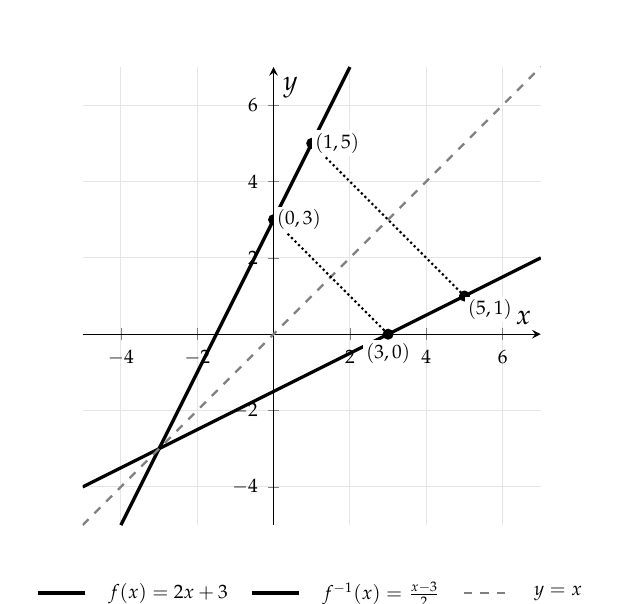
\begin{tikzpicture}
\begin{axis}[width=7.4cm,height=7.4cm,axis lines=middle,xmin=-5,xmax=7,ymin=-5,ymax=7,
  xtick={-4,-2,2,4,6},ytick={-4,-2,2,4,6},grid=major,grid style={gray!20},
  xlabel={$x$},ylabel={$y$},tick label style={font=\scriptsize},
  legend style={at={(0.5,-0.1)},anchor=north,font=\scriptsize,draw=none,legend columns=3,column sep=6pt}]
\addplot[FangBlue,very thick,domain=-4:2]{2*x+3}; \addlegendentry{$f(x)=2x+3$}
\addplot[FangRed,very thick,domain=-5:7]{(x-3)/2}; \addlegendentry{$\finv(x)=\frac{x-3}{2}$}
\addplot[dashed,gray,thick,domain=-5:7]{x}; \addlegendentry{$y=x$}
\draw[densely dotted,thick,FangPurple](axis cs:0,3)--(axis cs:3,0);
\draw[densely dotted,thick,FangPurple](axis cs:1,5)--(axis cs:5,1);
\fill[FangBlue](axis cs:0,3) circle(2pt) node[right,font=\scriptsize,fill=white,inner sep=1pt]{$(0,3)$};
\fill[FangRed](axis cs:3,0) circle(2pt) node[below,font=\scriptsize,fill=white,inner sep=1pt,yshift=-2pt]{$(3,0)$};
\fill[FangBlue](axis cs:1,5) circle(2pt) node[right,font=\scriptsize,fill=white,inner sep=1pt]{$(1,5)$};
\fill[FangRed](axis cs:5,1) circle(2pt) node[below right,font=\scriptsize,fill=white,inner sep=1pt]{$(5,1)$};
\end{axis}
\end{tikzpicture}\\[-2pt]
{\small\textbf{Figure 1.} Each point $(a,b)$ on $f$ has a partner $(b,a)$ on $\finv$.}
\end{minipage}\hfill
\begin{minipage}[t]{0.485\textwidth}\centering
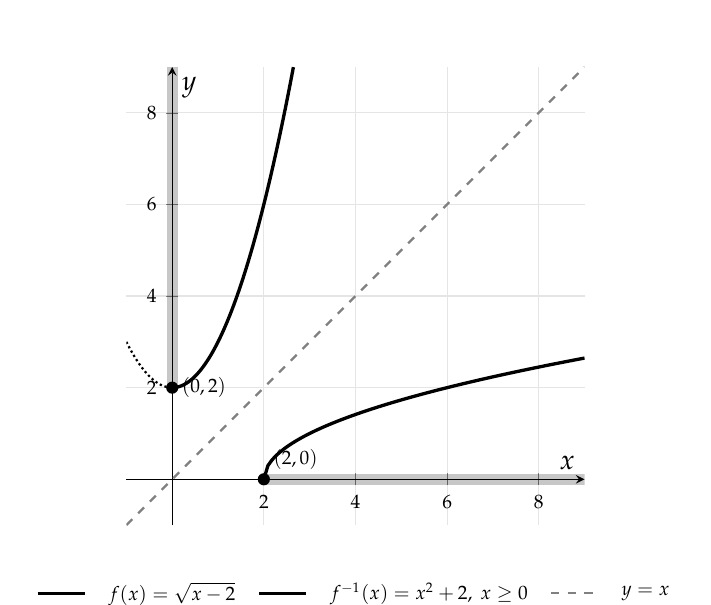
\begin{tikzpicture}
\begin{axis}[width=7.4cm,height=7.4cm,axis lines=middle,xmin=-1,xmax=9,ymin=-1,ymax=9,
  xtick={2,4,6,8},ytick={2,4,6,8},grid=major,grid style={gray!20},
  xlabel={$x$},ylabel={$y$},tick label style={font=\scriptsize},
  legend style={at={(0.5,-0.1)},anchor=north,font=\scriptsize,draw=none,legend columns=3,column sep=6pt}]
\draw[FangBlue,line width=4pt,opacity=0.22](axis cs:2,0)--(axis cs:9,0);
\draw[FangRed,line width=4pt,opacity=0.22](axis cs:0,2)--(axis cs:0,9);
\addplot[FangBlue,very thick,domain=2:9,samples=80]{sqrt(x-2)}; \addlegendentry{$f(x)=\sqrt{x-2}$}
\addplot[FangRed,very thick,domain=0:2.645,samples=60]{x^2+2}; \addlegendentry{$\finv(x)=x^2+2,\ x\ge0$}
\addplot[dashed,gray,thick,domain=-1:9]{x}; \addlegendentry{$y=x$}
\addplot[FangRed,thick,densely dotted,domain=-1:0,samples=30]{x^2+2};
\fill[FangBlue](axis cs:2,0) circle(2.2pt) node[above right,font=\scriptsize]{$(2,0)$};
\fill[FangRed](axis cs:0,2) circle(2.2pt) node[right,font=\scriptsize]{$(0,2)$};
\end{axis}
\end{tikzpicture}\\[-2pt]
{\small\textbf{Figure 2.} Shaded strips: domain of $f$ (blue) and range of $\finv$ (red).}
\end{minipage}
\end{center}

\begin{multicols}{2}
\textbf{Fold the paper along $y=x$:} the graph of $f$ lands exactly on the graph of $\finv$.\par
\textbf{Why?} The points $(a,b)$ and $(b,a)$ are mirror images in $y=x$:
\begin{itemize}[leftmargin=*,itemsep=1pt,topsep=2pt]
\item their midpoint $\left(\frac{a+b}{2},\frac{a+b}{2}\right)$ \textbf{lies on} $y=x$;
\item the segment joining them has slope $\frac{a-b}{b-a}=-1$, so it is \textbf{perpendicular} to $y=x$.
\end{itemize}
Every point of $f$ is reflected, so the whole graph is reflected. \textbf{Slope bonus:} $2$ and $\tfrac12$ are reciprocals — steep becomes flat.
\columnbreak

\textbf{Domain and range trade places, too} (Figure 2). \par
$f(x)=\sqrt{x-2}$: domain $[2,\infty)$, range $[0,\infty)$. \par
$\finv(x)=x^2+2$, $x\ge0$: domain $[0,\infty)$, range $[2,\infty)$. \par
The dotted left half of the parabola is \textbf{not} part of $\finv$ — it is not the mirror image of any point of $f$. That is why we wrote ``$x\ge0$'' in Example~3.
\end{multicols}

% ======================= PART 4 =======================
\sect{4}{Domain and range of the inverse}

\begin{idea}[The rule]
\[ \text{Domain of } \finv = \text{Range of } f \qquad\qquad \text{Range of } \finv = \text{Domain of } f \]
Reason: $\finv$ uses the outputs of $f$ as its inputs, and gives back the inputs of $f$ as its outputs.
\end{idea}

\textbf{How to find them — the safe method}
\begin{enumerate}[leftmargin=*,itemsep=2pt]
\item Find the domain and range of $f$ \textbf{first} (look at the graph, or ask ``which $x$ are allowed?'' and ``which $y$ can come out?'').
\item \textbf{Swap} them: that gives the domain and range of $\finv$.
\item Find the formula for $\finv$, then \textbf{attach the domain from step 2} to it.
\end{enumerate}

\begin{warn}
\textbf{Don't trust the formula alone.} In Example 3 the formula $x^2+2$ works for every real $x$, but the inverse only has domain $[0,\infty)$ — because that is the range of $f(x)=\sqrt{x-2}$. Always get the domain of $\finv$ from the range of $f$.
\end{warn}

\begin{example}[Example 4 \;·\; rational function]
$f(x)=\dfrac{2x+1}{x-3}$: domain $x\neq3$ (can't divide by $0$). Horizontal asymptote $y=\frac{2}{1}=2$, and $f(x)=2$ has no solution, so range $y\neq2$.\par
Therefore $\finv(x)=\dfrac{3x+1}{x-2}$ has \textbf{domain} $x\neq2$ and \textbf{range} $y\neq3$. The formula agrees: it is undefined at $x=2$, and its horizontal asymptote is $y=3$. \checkmark
\end{example}

\begin{example}[Example 5 \;·\; when there is no inverse — restrict the domain]
$f(x)=x^2$ is \textbf{not one-to-one}: $f(2)=f(-2)=4$, so $\finv(4)$ would have to be both $2$ and $-2$. On the graph, the horizontal line $y=4$ hits the parabola twice (\textbf{horizontal line test} fails).\par
Fix: keep only half. With domain $x\ge0$: range $[0,\infty)$, so $\finv(x)=\sqrt{x}$ with domain $[0,\infty)$ and range $[0,\infty)$.\par
With domain $x\le0$ instead: $\finv(x)=-\sqrt{x}$, domain $[0,\infty)$, range $(-\infty,0]$.
\end{example}

\begin{center}
\renewcommand{\arraystretch}{1.25}
\begin{tabular}{@{}lll@{}}
\toprule
\textbf{Question} & \textbf{About $f$} & \textbf{About $\finv$}\\ \midrule
Point & $(a,b)$ & $(b,a)$\\
Domain & $D$ & the range of $f$\\
Range & $R$ & the domain of $f$\\
Graph & — & reflection of $f$ over $y=x$\\
Exists? & only if $f$ is one-to-one & passes the horizontal line test\\
Proof & \multicolumn{2}{l}{$f(\finv(x))=x$ \textbf{and} $\finv(f(x))=x$}\\
\bottomrule
\end{tabular}
\end{center}

% ======================= PRACTICE =======================
\newpage
\sect{5}{Practice}
\ifkey\else\textit{Show your work. When you find an inverse, do a simple-case check: pick an easy $x$, find $f(x)$, and make sure $\finv$ sends it back.}\fi

\medskip
\needspace{6cm}{\large\bfseries\color{FangBlue}A.\ Warm-up} \easy

\begin{enumerate}[leftmargin=*,label=\textbf{\arabic*.},itemsep=6pt]
\np\item If $f(3)=7$, what is $\finv(7)$? \hfill If $\finv(-2)=5$, what is $f(5)$?
\work[1.2cm]{$\finv(7)=3$ (because $f$ sends $3$ to $7$). \quad $f(5)=-2$ (because $\finv$ sends $-2$ to $5$, so $f$ sends $5$ to $-2$).}

\np\item The table shows $f$. Find $\finv(11)$ and $\finv(5)$, and make a table for $\finv$.
\qquad\begin{tabular}{c|cccc}$x$&1&2&3&4\\\hline $f(x)$&5&8&11&14\end{tabular}
\work[1.6cm]{$\finv(11)=3$, \; $\finv(5)=1$. \quad Table of $\finv$: \; $x$: $5,8,11,14$ \;$\to$\; $\finv(x)$: $1,2,3,4$. \\ (Here $f(x)=3x+2$, so $\finv(x)=\frac{x-2}{3}$.)}

\np\item Find $\finv(x)$ for $f(x)=4x-5$.
\work[2.2cm]{$y=4x-5$ \;$\to$\; swap: $x=4y-5$ \;$\to$\; $x+5=4y$ \;$\to$\; $\finv(x)=\dfrac{x+5}{4}$. \; Check: $f(2)=3$, $\finv(3)=2$ \checkmark}

\np\item Find $\finv(x)$ for $f(x)=\dfrac{x+6}{3}$.
\work[2.2cm]{Swap: $x=\dfrac{y+6}{3}$ \;$\to$\; $3x=y+6$ \;$\to$\; $\finv(x)=3x-6$. \; Check: $f(0)=2$, $\finv(2)=0$ \checkmark}
\end{enumerate}

\needspace{6cm}{\large\bfseries\color{FangBlue}B.\ Prove it (check both orders)} \medium

\begin{enumerate}[resume,leftmargin=*,label=\textbf{\arabic*.},itemsep=6pt]
\np\item Prove that $f(x)=3x-7$ and $g(x)=\dfrac{x+7}{3}$ are inverses.
\work[2.6cm]{$f(g(x))=3\cdot\dfrac{x+7}{3}-7=x+7-7=x$. \quad $g(f(x))=\dfrac{(3x-7)+7}{3}=\dfrac{3x}{3}=x$. \\ Both are $x$ for all real $x$, so they are inverses. $\blacksquare$}

\np\item Are $f(x)=x^3+1$ and $g(x)=\sqrt[3]{x-1}$ inverses? Prove your answer.
\work[2.6cm]{$f(g(x))=\big(\sqrt[3]{x-1}\big)^3+1=(x-1)+1=x$. \quad $g(f(x))=\sqrt[3]{(x^3+1)-1}=\sqrt[3]{x^3}=x$. \\ Yes — both orders give $x$ for every real $x$ (cube roots work for negatives too). $\blacksquare$}

\np\item Are $f(x)=2x+4$ and $g(x)=\dfrac{x}{2}-4$ inverses? Prove your answer.
\work[2.4cm]{$f(g(x))=2\left(\dfrac{x}{2}-4\right)+4=x-8+4=x-4\neq x$. \; \textbf{Not} inverses (one failed composition is enough). \\ Simple case: $f(0)=4$ but $g(4)=-2\neq0$. The real inverse is $\finv(x)=\dfrac{x-4}{2}=\dfrac{x}{2}-2$.}
\end{enumerate}

\needspace{6cm}{\large\bfseries\color{FangBlue}C.\ Domain and range of $f$ and $\finv$} \medium\ \hard

\needspace{6cm}\textit{For each function: (a) domain and range of $f$, (b) the formula for $\finv$, (c) domain and range of $\finv$.}

\begin{enumerate}[resume,leftmargin=*,label=\textbf{\arabic*.},itemsep=6pt]
\np\item \medium\ $f(x)=\sqrt{x+3}$
\work[3.2cm]{(a) Domain $[-3,\infty)$ (need $x+3\ge0$); range $[0,\infty)$. \\
(b) Swap: $x=\sqrt{y+3}$ \;$\to$\; $x^2=y+3$ \;$\to$\; $\finv(x)=x^2-3$, \; $x\ge0$. \\
(c) Domain of $\finv$ $=[0,\infty)$ (the range of $f$); range of $\finv$ $=[-3,\infty)$ (the domain of $f$). \\
Check: $f(1)=2$, \; $\finv(2)=4-3=1$ \checkmark}

\np\item \medium\ $f(x)=(x-2)^2+1$, \; $x\ge2$
\work[3.2cm]{(a) Domain $[2,\infty)$ (given); the vertex is $(2,1)$ and the graph goes up, so range $[1,\infty)$. \\
(b) Swap: $x=(y-2)^2+1$ \;$\to$\; $(y-2)^2=x-1$ \;$\to$\; $y-2=\sqrt{x-1}$ (take $+$, because $y\ge2$) \;$\to$\; $\finv(x)=2+\sqrt{x-1}$. \\
(c) Domain of $\finv$ $=[1,\infty)$; range $=[2,\infty)$. \quad Check: $f(4)=5$, \; $\finv(5)=2+2=4$ \checkmark}

\np\item \medium\ $f(x)=\dfrac{x+1}{x-4}$
\work[3.4cm]{(a) Domain $x\neq4$. Horizontal asymptote $y=1$ and $f(x)=1$ has no solution, so range $y\neq1$. \\
(b) Swap: $x=\dfrac{y+1}{y-4}$ \;$\to$\; $xy-4x=y+1$ \;$\to$\; $xy-y=4x+1$ \;$\to$\; $y(x-1)=4x+1$ \;$\to$\; $\finv(x)=\dfrac{4x+1}{x-1}$. \\
(c) Domain of $\finv$: $x\neq1$; range: $y\neq4$ — exactly the range and domain of $f$ swapped. \quad Check: $f(5)=6$, $\finv(6)=\frac{25}{5}=5$ \checkmark}

\np\item \hard\ $f(x)=-\sqrt{4-x}$
\work[3.4cm]{(a) Need $4-x\ge0$: domain $(-\infty,4]$. A square root is $\ge0$, so with the minus sign: range $(-\infty,0]$. \\
(b) Swap: $x=-\sqrt{4-y}$ \;$\to$\; square: $x^2=4-y$ \;$\to$\; $\finv(x)=4-x^2$, \; $x\le0$. \\
(c) Domain of $\finv$ $=(-\infty,0]$; range $=(-\infty,4]$. \quad Check: $f(0)=-2$, \; $\finv(-2)=4-4=0$ \checkmark \\
(Without ``$x\le0$'' the formula would be a whole parabola — wrong.)}

\np\item \hard\ $f(x)=x^2-6x$ is not one-to-one. Restrict its domain to the largest interval that contains $x=5$ on which $f$ \emph{is} one-to-one. Then find $\finv$ with its domain and range.
\work[3.8cm]{Complete the square: $f(x)=(x-3)^2-9$, vertex $(3,-9)$. Each side of $x=3$ is one-to-one; the side containing $5$ is $x\ge3$. \\
$f$: domain $[3,\infty)$, range $[-9,\infty)$. \\
Swap: $x=(y-3)^2-9$ \;$\to$\; $(y-3)^2=x+9$ \;$\to$\; $y=3+\sqrt{x+9}$ (take $+$ because $y\ge3$). \\
$\finv(x)=3+\sqrt{x+9}$: domain $[-9,\infty)$, range $[3,\infty)$. \quad Check: $f(5)=-5$, \; $\finv(-5)=3+2=5$ \checkmark}
\end{enumerate}

\needspace{6cm}{\large\bfseries\color{FangBlue}D.\ Graphs} \medium

\begin{enumerate}[resume,leftmargin=*,label=\textbf{\arabic*.},itemsep=6pt]
\np\item The graph of $f$ is shown (blue, through $(-4,-3)$, $(-2,-2)$, $(0,0)$, $(2,4)$). Draw $y=x$, then sketch $\finv$ by swapping the coordinates of each marked point. State the domain and range of $f$ and of $\finv$.

\begin{center}
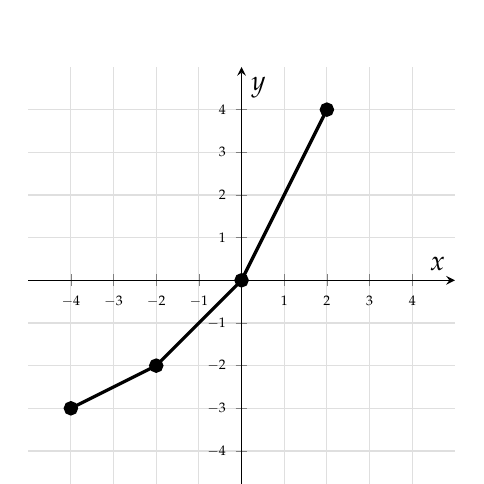
\begin{tikzpicture}
\begin{axis}[width=7cm,height=7cm,axis lines=middle,xmin=-5,xmax=5,ymin=-5,ymax=5,
  xtick={-4,...,4},ytick={-4,...,4},grid=both,grid style={gray!25},xlabel={$x$},ylabel={$y$},tick label style={font=\tiny}]
\addplot[FangBlue,very thick,mark=*,mark options={fill=FangBlue}] coordinates {(-4,-3)(-2,-2)(0,0)(2,4)};
\ifkey
\addplot[dashed,gray,thick,domain=-5:5]{x};
\addplot[FangRed,very thick,mark=*,mark options={fill=FangRed}] coordinates {(-3,-4)(-2,-2)(0,0)(4,2)};
\fi
\end{axis}
\end{tikzpicture}
\end{center}
\work[1.2cm]{$\finv$ (red) goes through $(-3,-4)$, $(-2,-2)$, $(0,0)$, $(4,2)$. Points on $y=x$, like $(-2,-2)$ and $(0,0)$, stay put. \\
$f$: domain $[-4,2]$, range $[-3,4]$. \quad $\finv$: domain $[-3,4]$, range $[-4,2]$.}

\np\item (a) The point $(-4,\,1)$ is on the graph of $f$. Which point must be on the graph of $\finv$? \\
(b) For $f(x)=2x-3$, find the point where the graphs of $f$ and $\finv$ cross.
\work[2.4cm]{(a) $(1,\,-4)$ — swap the coordinates. \\
(b) $\finv(x)=\dfrac{x+3}{2}$. The graphs are mirror images in $y=x$, so (for an increasing line) they meet on $y=x$: solve $2x-3=x$, so $x=3$. The point is $(3,3)$. Check: $f(3)=3$ and $\finv(3)=3$ \checkmark}
\end{enumerate}

\needspace{6cm}{\large\bfseries\color{FangBlue}E.\ Challenge} \hard

\begin{enumerate}[resume,leftmargin=*,label=\textbf{\arabic*.},itemsep=6pt]
\np\item Show that $f(x)=\dfrac{3x+2}{x-3}$ is its own inverse. What does that tell you about its graph?
\work[3.4cm]{$f(f(x))=\dfrac{3\cdot\frac{3x+2}{x-3}+2}{\frac{3x+2}{x-3}-3}=\dfrac{\frac{9x+6+2x-6}{x-3}}{\frac{3x+2-3x+9}{x-3}}=\dfrac{11x}{11}=x$ \; for $x\neq3$. \\
So $\finv=f$. Its graph is symmetric about the line $y=x$ (reflecting it changes nothing). Also: domain $x\neq3$ and range $y\neq3$ are the same set, as they must be.}

\np\item Explain why $f(x)=x^2$ has no inverse on all real numbers, but $g(x)=x^2$, $x\ge0$, does. Give the domain and range of $g^{-1}$.
\work[2.6cm]{$f(-2)=f(2)=4$: two inputs give the same output, so ``undo'' would have to send $4$ to two places — not a function (horizontal line test fails). Restricting to $x\ge0$ keeps each output only once. \\
$g^{-1}(x)=\sqrt{x}$: domain $[0,\infty)$ (range of $g$), range $[0,\infty)$ (domain of $g$).}
\end{enumerate}

\ifkey\else
\vfill
\begin{simple}
\textbf{Before you hand it in:} for every inverse you found, did you (1) check one easy number both ways, and (2) write the domain of $\finv$ as the \textbf{range of} $f$?
\end{simple}
\fi

\end{document}
"
% =====================================================================
\documentclass[11pt,letterpaper]{article}
\usepackage[margin=0.8in,top=0.85in,bottom=0.8in]{geometry}
\usepackage{mathpazo}
\usepackage[T1]{fontenc}
\usepackage{amsmath,amssymb}
\usepackage{xcolor}
\usepackage{enumitem}
\usepackage{multicol}
\usepackage{booktabs}
\usepackage{needspace}
\usepackage{fancyhdr}
\usepackage[most]{tcolorbox}
\usepackage{pgfplots}
\pgfplotsset{compat=1.17}
\usetikzlibrary{arrows.meta}

\definecolor{FangBlue}{HTML}{1F4E79}
\definecolor{FangTeal}{HTML}{0F7C7C}
\definecolor{FangGold}{HTML}{C9962B}
\definecolor{FangRed}{HTML}{B3261E}
\definecolor{FangGreen}{HTML}{2E8B57}
\definecolor{FangPurple}{HTML}{6A4BD8}
\definecolor{Soft}{HTML}{F4F7FB}
% black-and-white version: pdflatex with \def\isbw{1} before \input
\ifdefined\isbw
\definecolor{FangBlue}{HTML}{000000}\definecolor{FangTeal}{HTML}{000000}\definecolor{FangGold}{HTML}{555555}
\definecolor{FangRed}{HTML}{000000}\definecolor{FangGreen}{HTML}{000000}\definecolor{FangPurple}{HTML}{000000}\definecolor{Soft}{HTML}{FFFFFF}
\fi

\newif\ifkey
\ifdefined\iskey \keytrue \else \keyfalse \fi

\pagestyle{fancy}\fancyhf{}
\renewcommand{\headrulewidth}{0.4pt}
\fancyhead[L]{\small\color{FangBlue}\textbf{Prof. Fang Math} \,|\, Algebra 2 \,·\, 6-7 Inverse Relations \& Functions}
\fancyhead[R]{\small\ifkey\textcolor{FangRed}{\textbf{ANSWER KEY}}\else Name: \underline{\hspace{4.2cm}}\fi}
\fancyfoot[C]{\small\thepage}
\fancyfoot[R]{\scriptsize\color{gray}fangmath.com}
\setlength{\headheight}{14pt}
\setlength{\parindent}{0pt}
\setlength{\parskip}{4pt}

% ---------- boxes ----------
\newtcolorbox{idea}[1][]{colback=Soft,colframe=FangBlue,boxrule=0.8pt,arc=3pt,left=8pt,right=8pt,top=6pt,bottom=6pt,
  fonttitle=\bfseries,coltitle=white,colbacktitle=FangBlue,title={#1}}
\newtcolorbox{example}[1][]{colback=white,colframe=FangTeal,boxrule=0.6pt,arc=3pt,left=8pt,right=8pt,top=5pt,bottom=5pt,
  fonttitle=\bfseries,coltitle=FangTeal,colbacktitle=white,title={#1},attach boxed title to top left={xshift=8pt,yshift=-7pt},boxed title style={boxrule=0pt,colframe=white}, enhanced}
\newtcolorbox{warn}{colback=FangRed!5,colframe=FangRed,boxrule=0.6pt,arc=3pt,left=8pt,right=8pt,top=4pt,bottom=4pt,leftrule=3pt}
\newtcolorbox{simple}{colback=FangGold!10,colframe=FangGold,boxrule=0.6pt,arc=3pt,left=8pt,right=8pt,top=4pt,bottom=4pt,leftrule=3pt}
\newtcolorbox{sol}{colback=FangGreen!6,colframe=FangGreen,boxrule=0.5pt,arc=2pt,left=6pt,right=6pt,top=3pt,bottom=3pt,breakable}

\newcommand{\badge}[2]{\tcbox[on line,colback=#1,colframe=#1,coltext=white,boxrule=0pt,arc=6pt,left=4pt,right=4pt,top=1pt,bottom=1pt,fontupper=\scriptsize\bfseries]{#2}}
\newcommand{\easy}{\badge{FangGreen}{EASY}}
\newcommand{\medium}{\badge{FangTeal}{MEDIUM}}
\newcommand{\hard}{\badge{FangRed}{HARD}}
\newcommand{\finv}{f^{-1}}
\newcommand{\work}[2][]{\ifkey\begin{sol}#2\end{sol}\else\vspace*{#1}\fi}
\newcommand{\np}[1][6cm]{\needspace{#1}}
\newcommand{\sect}[2]{\par\needspace{7cm}\medskip{\Large\bfseries\color{FangBlue}\tcbox[on line,colback=FangBlue,colframe=FangBlue,coltext=white,arc=2pt,boxrule=0pt,left=5pt,right=5pt,top=1pt,bottom=1pt]{#1}\ #2}\par\smallskip}

\begin{document}

% ======================= TITLE =======================
\begin{center}
{\color{FangBlue}\Huge\bfseries Inverse Functions}\\[2pt]
{\large Undo the function — find it, prove it, graph it, and get its domain \& range}
\ifkey\\[3pt]{\color{FangRed}\large\bfseries Answer Key with complete solutions}\fi
\end{center}
\vspace{-4pt}

\begin{idea}[The big idea]
A function $f$ takes an input $x$ to an output $y$. Its \textbf{inverse} $\finv$ goes back: it takes $y$ to $x$.
\[ x \xrightarrow{\;\;f\;\;} y \qquad\qquad y \xrightarrow{\;\;\finv\;\;} x \qquad\qquad\text{so}\qquad f(a)=b \iff \finv(b)=a. \]
Every point $(a,b)$ on $f$ becomes the point $(b,a)$ on $\finv$: \textbf{inputs and outputs trade places.}
\end{idea}

\begin{simple}
\textbf{Simple case first.} ``Add $3$'' is undone by ``subtract $3$'': if $f(x)=x+3$ then $\finv(x)=x-3$. Check: $f(4)=7$ and $\finv(7)=4$.\par
``Double, then add $3$'' is undone by doing the opposite steps in the \textbf{opposite order}: subtract $3$, then halve. Like putting on socks then shoes — you take off the shoes first.
\end{simple}

\begin{center}
\begin{tabular}{c|cccc}
\toprule
$x$ & $0$ & $1$ & $2$ & $3$\\ \midrule
$f(x)=2x+3$ & $3$ & $5$ & $7$ & $9$\\
\bottomrule
\end{tabular}
\qquad$\Longrightarrow$\qquad
\begin{tabular}{c|cccc}
\toprule
$x$ & $3$ & $5$ & $7$ & $9$\\ \midrule
$\finv(x)$ & $0$ & $1$ & $2$ & $3$\\
\bottomrule
\end{tabular}
\end{center}

\begin{warn}
\textbf{Watch out:} $\finv(x)$ means the \emph{inverse function}. It is \textbf{not} $\dfrac{1}{f(x)}$. The $-1$ is not an exponent here.
\end{warn}

% ======================= PART 1 =======================
\sect{1}{How to find the inverse — four steps}

\begin{multicols}{2}
\begin{enumerate}[leftmargin=*,itemsep=2pt]
\item Replace $f(x)$ with $y$.
\item \textbf{Swap} $x$ and $y$.
\item \textbf{Solve} for $y$.
\item Replace $y$ with $\finv(x)$ and \textbf{state its domain}.
\end{enumerate}
\columnbreak
Step 2 is the whole idea: swapping $x$ and $y$ is exactly ``inputs and outputs trade places.'' Steps 3 and 4 just tidy up the answer.
\end{multicols}

\begin{example}[Example 1 \;·\; a line]
Find the inverse of $f(x)=2x+3$.\par
\begin{tabular}{@{}ll@{}}
$y = 2x+3$ & Step 1\\
$x = 2y+3$ & Step 2: swap\\
$x-3 = 2y \;\Rightarrow\; y=\dfrac{x-3}{2}$ & Step 3: solve\\[6pt]
$\finv(x)=\dfrac{x-3}{2}$, \; domain: all real numbers & Step 4
\end{tabular}\par
\textbf{Simple case check:} $f(1)=5$, and $\finv(5)=\frac{5-3}{2}=1$. \checkmark
\end{example}

\begin{example}[Example 2 \;·\; a rational function]
Find the inverse of $f(x)=\dfrac{2x+1}{x-3}$.\par
Swap: $x=\dfrac{2y+1}{y-3}$. \; Multiply by $(y-3)$: $xy-3x=2y+1$. \; Collect the $y$ terms on one side: $xy-2y=3x+1$.\par
Factor out $y$: $y(x-2)=3x+1$, so
\[\finv(x)=\frac{3x+1}{x-2},\qquad x\neq 2.\]
\textbf{Simple case check:} $f(4)=\frac{9}{1}=9$, and $\finv(9)=\frac{28}{7}=4$. \checkmark
\end{example}

\begin{example}[Example 3 \;·\; a square root — the domain matters]
Find the inverse of $f(x)=\sqrt{x-2}$.\par
Swap: $x=\sqrt{y-2}$. Square both sides: $x^2=y-2$, so $y=x^2+2$.\par
\textbf{But} $x$ here was a square-root output, and square roots are never negative, so $x\ge 0$:
\[\finv(x)=x^2+2,\qquad x\ge 0.\]
Without ``$x\ge0$'' you would get a whole parabola, which is \emph{not} the inverse (see the graph in Part~3).
\end{example}

% ======================= PART 2 =======================
\sect{2}{How to prove two functions are inverses}

\begin{idea}[The test — you must check BOTH orders]
$f$ and $g$ are inverse functions exactly when
\[ f\big(g(x)\big)=x \ \text{ for every } x \text{ in the domain of } g \qquad\text{and}\qquad g\big(f(x)\big)=x \ \text{ for every } x \text{ in the domain of } f. \]
In words: doing one and then the other \textbf{always brings you back to where you started}.
\end{idea}

\textbf{Why this is the right test.} Suppose $f(a)=b$. If $g$ undoes $f$, then $g(b)=a$, i.e.\ $g(f(a))=a$. The same thinking with the roles switched gives $f(g(b))=b$. So ``undoing'' means exactly the two equations above.

\begin{example}[Proof 1 \;·\; $f(x)=2x+3$ and $g(x)=\dfrac{x-3}{2}$]
\[ f\big(g(x)\big)=2\cdot\frac{x-3}{2}+3=(x-3)+3=x. \qquad
   g\big(f(x)\big)=\frac{(2x+3)-3}{2}=\frac{2x}{2}=x. \]
Both compositions equal $x$ for all real $x$, so $g=\finv$. \qquad $\blacksquare$
\end{example}

\begin{example}[Proof 2 \;·\; $f(x)=\dfrac{2x+1}{x-3}$ and $g(x)=\dfrac{3x+1}{x-2}$]
\[ f\big(g(x)\big)=\frac{2\cdot\frac{3x+1}{x-2}+1}{\frac{3x+1}{x-2}-3}
 =\frac{\frac{2(3x+1)+(x-2)}{x-2}}{\frac{(3x+1)-3(x-2)}{x-2}}
 =\frac{6x+2+x-2}{3x+1-3x+6}=\frac{7x}{7}=x \quad (x\neq2). \]
\[ g\big(f(x)\big)=\frac{3\cdot\frac{2x+1}{x-3}+1}{\frac{2x+1}{x-3}-2}
 =\frac{\frac{3(2x+1)+(x-3)}{x-3}}{\frac{(2x+1)-2(x-3)}{x-3}}
 =\frac{6x+3+x-3}{2x+1-2x+6}=\frac{7x}{7}=x \quad (x\neq3). \]
Both orders give $x$, so they are inverses. \qquad $\blacksquare$
\end{example}

\begin{warn}
\textbf{Why one order is not enough.} Take $f(x)=x^2$ and $g(x)=\sqrt{x}$. Then $f(g(x))=(\sqrt x)^2=x$ for $x\ge0$ — looks fine. But $g(f(x))=\sqrt{x^2}=|x|$, and $g(f(-3))=3\neq-3$. So they are \textbf{not} inverses — unless we restrict $f$ to $x\ge0$ (Part 4).
\end{warn}

% ======================= PART 3 =======================
\sect{3}{The graph: a mirror image over the line $y=x$}

\begin{center}
\begin{minipage}[t]{0.485\textwidth}\centering
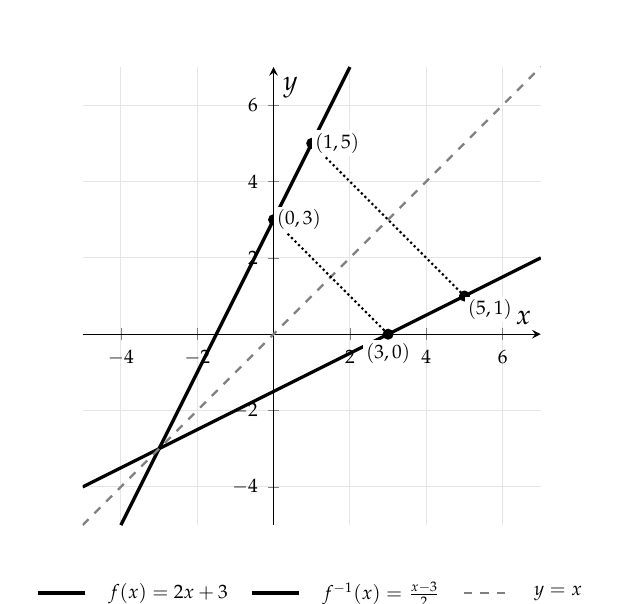
\begin{tikzpicture}
\begin{axis}[width=7.4cm,height=7.4cm,axis lines=middle,xmin=-5,xmax=7,ymin=-5,ymax=7,
  xtick={-4,-2,2,4,6},ytick={-4,-2,2,4,6},grid=major,grid style={gray!20},
  xlabel={$x$},ylabel={$y$},tick label style={font=\scriptsize},
  legend style={at={(0.5,-0.1)},anchor=north,font=\scriptsize,draw=none,legend columns=3,column sep=6pt}]
\addplot[FangBlue,very thick,domain=-4:2]{2*x+3}; \addlegendentry{$f(x)=2x+3$}
\addplot[FangRed,very thick,domain=-5:7]{(x-3)/2}; \addlegendentry{$\finv(x)=\frac{x-3}{2}$}
\addplot[dashed,gray,thick,domain=-5:7]{x}; \addlegendentry{$y=x$}
\draw[densely dotted,thick,FangPurple](axis cs:0,3)--(axis cs:3,0);
\draw[densely dotted,thick,FangPurple](axis cs:1,5)--(axis cs:5,1);
\fill[FangBlue](axis cs:0,3) circle(2pt) node[right,font=\scriptsize,fill=white,inner sep=1pt]{$(0,3)$};
\fill[FangRed](axis cs:3,0) circle(2pt) node[below,font=\scriptsize,fill=white,inner sep=1pt,yshift=-2pt]{$(3,0)$};
\fill[FangBlue](axis cs:1,5) circle(2pt) node[right,font=\scriptsize,fill=white,inner sep=1pt]{$(1,5)$};
\fill[FangRed](axis cs:5,1) circle(2pt) node[below right,font=\scriptsize,fill=white,inner sep=1pt]{$(5,1)$};
\end{axis}
\end{tikzpicture}\\[-2pt]
{\small\textbf{Figure 1.} Each point $(a,b)$ on $f$ has a partner $(b,a)$ on $\finv$.}
\end{minipage}\hfill
\begin{minipage}[t]{0.485\textwidth}\centering
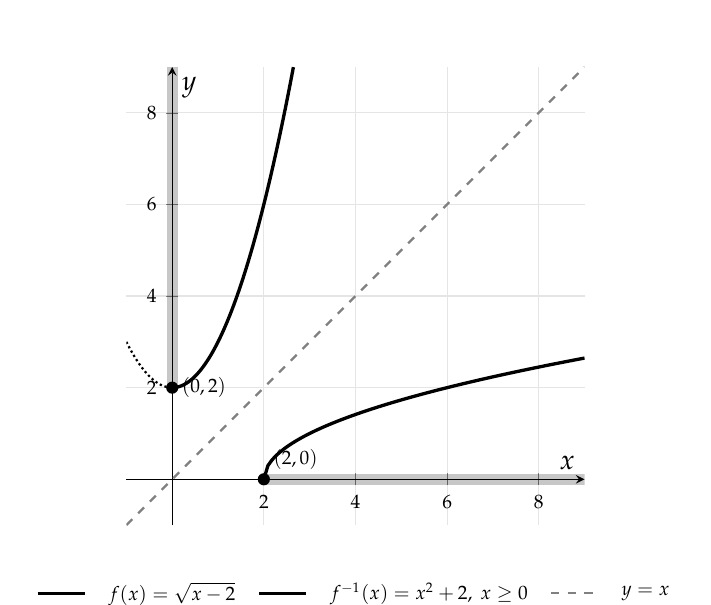
\begin{tikzpicture}
\begin{axis}[width=7.4cm,height=7.4cm,axis lines=middle,xmin=-1,xmax=9,ymin=-1,ymax=9,
  xtick={2,4,6,8},ytick={2,4,6,8},grid=major,grid style={gray!20},
  xlabel={$x$},ylabel={$y$},tick label style={font=\scriptsize},
  legend style={at={(0.5,-0.1)},anchor=north,font=\scriptsize,draw=none,legend columns=3,column sep=6pt}]
\draw[FangBlue,line width=4pt,opacity=0.22](axis cs:2,0)--(axis cs:9,0);
\draw[FangRed,line width=4pt,opacity=0.22](axis cs:0,2)--(axis cs:0,9);
\addplot[FangBlue,very thick,domain=2:9,samples=80]{sqrt(x-2)}; \addlegendentry{$f(x)=\sqrt{x-2}$}
\addplot[FangRed,very thick,domain=0:2.645,samples=60]{x^2+2}; \addlegendentry{$\finv(x)=x^2+2,\ x\ge0$}
\addplot[dashed,gray,thick,domain=-1:9]{x}; \addlegendentry{$y=x$}
\addplot[FangRed,thick,densely dotted,domain=-1:0,samples=30]{x^2+2};
\fill[FangBlue](axis cs:2,0) circle(2.2pt) node[above right,font=\scriptsize]{$(2,0)$};
\fill[FangRed](axis cs:0,2) circle(2.2pt) node[right,font=\scriptsize]{$(0,2)$};
\end{axis}
\end{tikzpicture}\\[-2pt]
{\small\textbf{Figure 2.} Shaded strips: domain of $f$ (blue) and range of $\finv$ (red).}
\end{minipage}
\end{center}

\begin{multicols}{2}
\textbf{Fold the paper along $y=x$:} the graph of $f$ lands exactly on the graph of $\finv$.\par
\textbf{Why?} The points $(a,b)$ and $(b,a)$ are mirror images in $y=x$:
\begin{itemize}[leftmargin=*,itemsep=1pt,topsep=2pt]
\item their midpoint $\left(\frac{a+b}{2},\frac{a+b}{2}\right)$ \textbf{lies on} $y=x$;
\item the segment joining them has slope $\frac{a-b}{b-a}=-1$, so it is \textbf{perpendicular} to $y=x$.
\end{itemize}
Every point of $f$ is reflected, so the whole graph is reflected. \textbf{Slope bonus:} $2$ and $\tfrac12$ are reciprocals — steep becomes flat.
\columnbreak

\textbf{Domain and range trade places, too} (Figure 2). \par
$f(x)=\sqrt{x-2}$: domain $[2,\infty)$, range $[0,\infty)$. \par
$\finv(x)=x^2+2$, $x\ge0$: domain $[0,\infty)$, range $[2,\infty)$. \par
The dotted left half of the parabola is \textbf{not} part of $\finv$ — it is not the mirror image of any point of $f$. That is why we wrote ``$x\ge0$'' in Example~3.
\end{multicols}

% ======================= PART 4 =======================
\sect{4}{Domain and range of the inverse}

\begin{idea}[The rule]
\[ \text{Domain of } \finv = \text{Range of } f \qquad\qquad \text{Range of } \finv = \text{Domain of } f \]
Reason: $\finv$ uses the outputs of $f$ as its inputs, and gives back the inputs of $f$ as its outputs.
\end{idea}

\textbf{How to find them — the safe method}
\begin{enumerate}[leftmargin=*,itemsep=2pt]
\item Find the domain and range of $f$ \textbf{first} (look at the graph, or ask ``which $x$ are allowed?'' and ``which $y$ can come out?'').
\item \textbf{Swap} them: that gives the domain and range of $\finv$.
\item Find the formula for $\finv$, then \textbf{attach the domain from step 2} to it.
\end{enumerate}

\begin{warn}
\textbf{Don't trust the formula alone.} In Example 3 the formula $x^2+2$ works for every real $x$, but the inverse only has domain $[0,\infty)$ — because that is the range of $f(x)=\sqrt{x-2}$. Always get the domain of $\finv$ from the range of $f$.
\end{warn}

\begin{example}[Example 4 \;·\; rational function]
$f(x)=\dfrac{2x+1}{x-3}$: domain $x\neq3$ (can't divide by $0$). Horizontal asymptote $y=\frac{2}{1}=2$, and $f(x)=2$ has no solution, so range $y\neq2$.\par
Therefore $\finv(x)=\dfrac{3x+1}{x-2}$ has \textbf{domain} $x\neq2$ and \textbf{range} $y\neq3$. The formula agrees: it is undefined at $x=2$, and its horizontal asymptote is $y=3$. \checkmark
\end{example}

\begin{example}[Example 5 \;·\; when there is no inverse — restrict the domain]
$f(x)=x^2$ is \textbf{not one-to-one}: $f(2)=f(-2)=4$, so $\finv(4)$ would have to be both $2$ and $-2$. On the graph, the horizontal line $y=4$ hits the parabola twice (\textbf{horizontal line test} fails).\par
Fix: keep only half. With domain $x\ge0$: range $[0,\infty)$, so $\finv(x)=\sqrt{x}$ with domain $[0,\infty)$ and range $[0,\infty)$.\par
With domain $x\le0$ instead: $\finv(x)=-\sqrt{x}$, domain $[0,\infty)$, range $(-\infty,0]$.
\end{example}

\begin{center}
\renewcommand{\arraystretch}{1.25}
\begin{tabular}{@{}lll@{}}
\toprule
\textbf{Question} & \textbf{About $f$} & \textbf{About $\finv$}\\ \midrule
Point & $(a,b)$ & $(b,a)$\\
Domain & $D$ & the range of $f$\\
Range & $R$ & the domain of $f$\\
Graph & — & reflection of $f$ over $y=x$\\
Exists? & only if $f$ is one-to-one & passes the horizontal line test\\
Proof & \multicolumn{2}{l}{$f(\finv(x))=x$ \textbf{and} $\finv(f(x))=x$}\\
\bottomrule
\end{tabular}
\end{center}

% ======================= PRACTICE =======================
\newpage
\sect{5}{Practice}
\ifkey\else\textit{Show your work. When you find an inverse, do a simple-case check: pick an easy $x$, find $f(x)$, and make sure $\finv$ sends it back.}\fi

\medskip
\needspace{6cm}{\large\bfseries\color{FangBlue}A.\ Warm-up} \easy

\begin{enumerate}[leftmargin=*,label=\textbf{\arabic*.},itemsep=6pt]
\np\item If $f(3)=7$, what is $\finv(7)$? \hfill If $\finv(-2)=5$, what is $f(5)$?
\work[1.2cm]{$\finv(7)=3$ (because $f$ sends $3$ to $7$). \quad $f(5)=-2$ (because $\finv$ sends $-2$ to $5$, so $f$ sends $5$ to $-2$).}

\np\item The table shows $f$. Find $\finv(11)$ and $\finv(5)$, and make a table for $\finv$.
\qquad\begin{tabular}{c|cccc}$x$&1&2&3&4\\\hline $f(x)$&5&8&11&14\end{tabular}
\work[1.6cm]{$\finv(11)=3$, \; $\finv(5)=1$. \quad Table of $\finv$: \; $x$: $5,8,11,14$ \;$\to$\; $\finv(x)$: $1,2,3,4$. \\ (Here $f(x)=3x+2$, so $\finv(x)=\frac{x-2}{3}$.)}

\np\item Find $\finv(x)$ for $f(x)=4x-5$.
\work[2.2cm]{$y=4x-5$ \;$\to$\; swap: $x=4y-5$ \;$\to$\; $x+5=4y$ \;$\to$\; $\finv(x)=\dfrac{x+5}{4}$. \; Check: $f(2)=3$, $\finv(3)=2$ \checkmark}

\np\item Find $\finv(x)$ for $f(x)=\dfrac{x+6}{3}$.
\work[2.2cm]{Swap: $x=\dfrac{y+6}{3}$ \;$\to$\; $3x=y+6$ \;$\to$\; $\finv(x)=3x-6$. \; Check: $f(0)=2$, $\finv(2)=0$ \checkmark}
\end{enumerate}

\needspace{6cm}{\large\bfseries\color{FangBlue}B.\ Prove it (check both orders)} \medium

\begin{enumerate}[resume,leftmargin=*,label=\textbf{\arabic*.},itemsep=6pt]
\np\item Prove that $f(x)=3x-7$ and $g(x)=\dfrac{x+7}{3}$ are inverses.
\work[2.6cm]{$f(g(x))=3\cdot\dfrac{x+7}{3}-7=x+7-7=x$. \quad $g(f(x))=\dfrac{(3x-7)+7}{3}=\dfrac{3x}{3}=x$. \\ Both are $x$ for all real $x$, so they are inverses. $\blacksquare$}

\np\item Are $f(x)=x^3+1$ and $g(x)=\sqrt[3]{x-1}$ inverses? Prove your answer.
\work[2.6cm]{$f(g(x))=\big(\sqrt[3]{x-1}\big)^3+1=(x-1)+1=x$. \quad $g(f(x))=\sqrt[3]{(x^3+1)-1}=\sqrt[3]{x^3}=x$. \\ Yes — both orders give $x$ for every real $x$ (cube roots work for negatives too). $\blacksquare$}

\np\item Are $f(x)=2x+4$ and $g(x)=\dfrac{x}{2}-4$ inverses? Prove your answer.
\work[2.4cm]{$f(g(x))=2\left(\dfrac{x}{2}-4\right)+4=x-8+4=x-4\neq x$. \; \textbf{Not} inverses (one failed composition is enough). \\ Simple case: $f(0)=4$ but $g(4)=-2\neq0$. The real inverse is $\finv(x)=\dfrac{x-4}{2}=\dfrac{x}{2}-2$.}
\end{enumerate}

\needspace{6cm}{\large\bfseries\color{FangBlue}C.\ Domain and range of $f$ and $\finv$} \medium\ \hard

\needspace{6cm}\textit{For each function: (a) domain and range of $f$, (b) the formula for $\finv$, (c) domain and range of $\finv$.}

\begin{enumerate}[resume,leftmargin=*,label=\textbf{\arabic*.},itemsep=6pt]
\np\item \medium\ $f(x)=\sqrt{x+3}$
\work[3.2cm]{(a) Domain $[-3,\infty)$ (need $x+3\ge0$); range $[0,\infty)$. \\
(b) Swap: $x=\sqrt{y+3}$ \;$\to$\; $x^2=y+3$ \;$\to$\; $\finv(x)=x^2-3$, \; $x\ge0$. \\
(c) Domain of $\finv$ $=[0,\infty)$ (the range of $f$); range of $\finv$ $=[-3,\infty)$ (the domain of $f$). \\
Check: $f(1)=2$, \; $\finv(2)=4-3=1$ \checkmark}

\np\item \medium\ $f(x)=(x-2)^2+1$, \; $x\ge2$
\work[3.2cm]{(a) Domain $[2,\infty)$ (given); the vertex is $(2,1)$ and the graph goes up, so range $[1,\infty)$. \\
(b) Swap: $x=(y-2)^2+1$ \;$\to$\; $(y-2)^2=x-1$ \;$\to$\; $y-2=\sqrt{x-1}$ (take $+$, because $y\ge2$) \;$\to$\; $\finv(x)=2+\sqrt{x-1}$. \\
(c) Domain of $\finv$ $=[1,\infty)$; range $=[2,\infty)$. \quad Check: $f(4)=5$, \; $\finv(5)=2+2=4$ \checkmark}

\np\item \medium\ $f(x)=\dfrac{x+1}{x-4}$
\work[3.4cm]{(a) Domain $x\neq4$. Horizontal asymptote $y=1$ and $f(x)=1$ has no solution, so range $y\neq1$. \\
(b) Swap: $x=\dfrac{y+1}{y-4}$ \;$\to$\; $xy-4x=y+1$ \;$\to$\; $xy-y=4x+1$ \;$\to$\; $y(x-1)=4x+1$ \;$\to$\; $\finv(x)=\dfrac{4x+1}{x-1}$. \\
(c) Domain of $\finv$: $x\neq1$; range: $y\neq4$ — exactly the range and domain of $f$ swapped. \quad Check: $f(5)=6$, $\finv(6)=\frac{25}{5}=5$ \checkmark}

\np\item \hard\ $f(x)=-\sqrt{4-x}$
\work[3.4cm]{(a) Need $4-x\ge0$: domain $(-\infty,4]$. A square root is $\ge0$, so with the minus sign: range $(-\infty,0]$. \\
(b) Swap: $x=-\sqrt{4-y}$ \;$\to$\; square: $x^2=4-y$ \;$\to$\; $\finv(x)=4-x^2$, \; $x\le0$. \\
(c) Domain of $\finv$ $=(-\infty,0]$; range $=(-\infty,4]$. \quad Check: $f(0)=-2$, \; $\finv(-2)=4-4=0$ \checkmark \\
(Without ``$x\le0$'' the formula would be a whole parabola — wrong.)}

\np\item \hard\ $f(x)=x^2-6x$ is not one-to-one. Restrict its domain to the largest interval that contains $x=5$ on which $f$ \emph{is} one-to-one. Then find $\finv$ with its domain and range.
\work[3.8cm]{Complete the square: $f(x)=(x-3)^2-9$, vertex $(3,-9)$. Each side of $x=3$ is one-to-one; the side containing $5$ is $x\ge3$. \\
$f$: domain $[3,\infty)$, range $[-9,\infty)$. \\
Swap: $x=(y-3)^2-9$ \;$\to$\; $(y-3)^2=x+9$ \;$\to$\; $y=3+\sqrt{x+9}$ (take $+$ because $y\ge3$). \\
$\finv(x)=3+\sqrt{x+9}$: domain $[-9,\infty)$, range $[3,\infty)$. \quad Check: $f(5)=-5$, \; $\finv(-5)=3+2=5$ \checkmark}
\end{enumerate}

\needspace{6cm}{\large\bfseries\color{FangBlue}D.\ Graphs} \medium

\begin{enumerate}[resume,leftmargin=*,label=\textbf{\arabic*.},itemsep=6pt]
\np\item The graph of $f$ is shown (blue, through $(-4,-3)$, $(-2,-2)$, $(0,0)$, $(2,4)$). Draw $y=x$, then sketch $\finv$ by swapping the coordinates of each marked point. State the domain and range of $f$ and of $\finv$.

\begin{center}
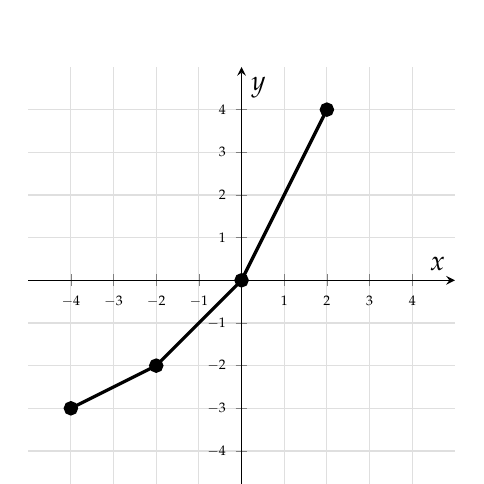
\begin{tikzpicture}
\begin{axis}[width=7cm,height=7cm,axis lines=middle,xmin=-5,xmax=5,ymin=-5,ymax=5,
  xtick={-4,...,4},ytick={-4,...,4},grid=both,grid style={gray!25},xlabel={$x$},ylabel={$y$},tick label style={font=\tiny}]
\addplot[FangBlue,very thick,mark=*,mark options={fill=FangBlue}] coordinates {(-4,-3)(-2,-2)(0,0)(2,4)};
\ifkey
\addplot[dashed,gray,thick,domain=-5:5]{x};
\addplot[FangRed,very thick,mark=*,mark options={fill=FangRed}] coordinates {(-3,-4)(-2,-2)(0,0)(4,2)};
\fi
\end{axis}
\end{tikzpicture}
\end{center}
\work[1.2cm]{$\finv$ (red) goes through $(-3,-4)$, $(-2,-2)$, $(0,0)$, $(4,2)$. Points on $y=x$, like $(-2,-2)$ and $(0,0)$, stay put. \\
$f$: domain $[-4,2]$, range $[-3,4]$. \quad $\finv$: domain $[-3,4]$, range $[-4,2]$.}

\np\item (a) The point $(-4,\,1)$ is on the graph of $f$. Which point must be on the graph of $\finv$? \\
(b) For $f(x)=2x-3$, find the point where the graphs of $f$ and $\finv$ cross.
\work[2.4cm]{(a) $(1,\,-4)$ — swap the coordinates. \\
(b) $\finv(x)=\dfrac{x+3}{2}$. The graphs are mirror images in $y=x$, so (for an increasing line) they meet on $y=x$: solve $2x-3=x$, so $x=3$. The point is $(3,3)$. Check: $f(3)=3$ and $\finv(3)=3$ \checkmark}
\end{enumerate}

\needspace{6cm}{\large\bfseries\color{FangBlue}E.\ Challenge} \hard

\begin{enumerate}[resume,leftmargin=*,label=\textbf{\arabic*.},itemsep=6pt]
\np\item Show that $f(x)=\dfrac{3x+2}{x-3}$ is its own inverse. What does that tell you about its graph?
\work[3.4cm]{$f(f(x))=\dfrac{3\cdot\frac{3x+2}{x-3}+2}{\frac{3x+2}{x-3}-3}=\dfrac{\frac{9x+6+2x-6}{x-3}}{\frac{3x+2-3x+9}{x-3}}=\dfrac{11x}{11}=x$ \; for $x\neq3$. \\
So $\finv=f$. Its graph is symmetric about the line $y=x$ (reflecting it changes nothing). Also: domain $x\neq3$ and range $y\neq3$ are the same set, as they must be.}

\np\item Explain why $f(x)=x^2$ has no inverse on all real numbers, but $g(x)=x^2$, $x\ge0$, does. Give the domain and range of $g^{-1}$.
\work[2.6cm]{$f(-2)=f(2)=4$: two inputs give the same output, so ``undo'' would have to send $4$ to two places — not a function (horizontal line test fails). Restricting to $x\ge0$ keeps each output only once. \\
$g^{-1}(x)=\sqrt{x}$: domain $[0,\infty)$ (range of $g$), range $[0,\infty)$ (domain of $g$).}
\end{enumerate}

\ifkey\else
\vfill
\begin{simple}
\textbf{Before you hand it in:} for every inverse you found, did you (1) check one easy number both ways, and (2) write the domain of $\finv$ as the \textbf{range of} $f$?
\end{simple}
\fi

\end{document}
"
% =====================================================================
\documentclass[11pt,letterpaper]{article}
\usepackage[margin=0.8in,top=0.85in,bottom=0.8in]{geometry}
\usepackage{mathpazo}
\usepackage[T1]{fontenc}
\usepackage{amsmath,amssymb}
\usepackage{xcolor}
\usepackage{enumitem}
\usepackage{multicol}
\usepackage{booktabs}
\usepackage{needspace}
\usepackage{fancyhdr}
\usepackage[most]{tcolorbox}
\usepackage{pgfplots}
\pgfplotsset{compat=1.17}
\usetikzlibrary{arrows.meta}

\definecolor{FangBlue}{HTML}{1F4E79}
\definecolor{FangTeal}{HTML}{0F7C7C}
\definecolor{FangGold}{HTML}{C9962B}
\definecolor{FangRed}{HTML}{B3261E}
\definecolor{FangGreen}{HTML}{2E8B57}
\definecolor{FangPurple}{HTML}{6A4BD8}
\definecolor{Soft}{HTML}{F4F7FB}
% black-and-white version: pdflatex with \def\isbw{1} before \input
\ifdefined\isbw
\definecolor{FangBlue}{HTML}{000000}\definecolor{FangTeal}{HTML}{000000}\definecolor{FangGold}{HTML}{555555}
\definecolor{FangRed}{HTML}{000000}\definecolor{FangGreen}{HTML}{000000}\definecolor{FangPurple}{HTML}{000000}\definecolor{Soft}{HTML}{FFFFFF}
\fi

\newif\ifkey
\ifdefined\iskey \keytrue \else \keyfalse \fi

\pagestyle{fancy}\fancyhf{}
\renewcommand{\headrulewidth}{0.4pt}
\fancyhead[L]{\small\color{FangBlue}\textbf{Prof. Fang Math} \,|\, Algebra 2 \,·\, 6-7 Inverse Relations \& Functions}
\fancyhead[R]{\small\ifkey\textcolor{FangRed}{\textbf{ANSWER KEY}}\else Name: \underline{\hspace{4.2cm}}\fi}
\fancyfoot[C]{\small\thepage}
\fancyfoot[R]{\scriptsize\color{gray}fangmath.com}
\setlength{\headheight}{14pt}
\setlength{\parindent}{0pt}
\setlength{\parskip}{4pt}

% ---------- boxes ----------
\newtcolorbox{idea}[1][]{colback=Soft,colframe=FangBlue,boxrule=0.8pt,arc=3pt,left=8pt,right=8pt,top=6pt,bottom=6pt,
  fonttitle=\bfseries,coltitle=white,colbacktitle=FangBlue,title={#1}}
\newtcolorbox{example}[1][]{colback=white,colframe=FangTeal,boxrule=0.6pt,arc=3pt,left=8pt,right=8pt,top=5pt,bottom=5pt,
  fonttitle=\bfseries,coltitle=FangTeal,colbacktitle=white,title={#1},attach boxed title to top left={xshift=8pt,yshift=-7pt},boxed title style={boxrule=0pt,colframe=white}, enhanced}
\newtcolorbox{warn}{colback=FangRed!5,colframe=FangRed,boxrule=0.6pt,arc=3pt,left=8pt,right=8pt,top=4pt,bottom=4pt,leftrule=3pt}
\newtcolorbox{simple}{colback=FangGold!10,colframe=FangGold,boxrule=0.6pt,arc=3pt,left=8pt,right=8pt,top=4pt,bottom=4pt,leftrule=3pt}
\newtcolorbox{sol}{colback=FangGreen!6,colframe=FangGreen,boxrule=0.5pt,arc=2pt,left=6pt,right=6pt,top=3pt,bottom=3pt,breakable}

\newcommand{\badge}[2]{\tcbox[on line,colback=#1,colframe=#1,coltext=white,boxrule=0pt,arc=6pt,left=4pt,right=4pt,top=1pt,bottom=1pt,fontupper=\scriptsize\bfseries]{#2}}
\newcommand{\easy}{\badge{FangGreen}{EASY}}
\newcommand{\medium}{\badge{FangTeal}{MEDIUM}}
\newcommand{\hard}{\badge{FangRed}{HARD}}
\newcommand{\finv}{f^{-1}}
\newcommand{\work}[2][]{\ifkey\begin{sol}#2\end{sol}\else\vspace*{#1}\fi}
\newcommand{\np}[1][6cm]{\needspace{#1}}
\newcommand{\sect}[2]{\par\needspace{7cm}\medskip{\Large\bfseries\color{FangBlue}\tcbox[on line,colback=FangBlue,colframe=FangBlue,coltext=white,arc=2pt,boxrule=0pt,left=5pt,right=5pt,top=1pt,bottom=1pt]{#1}\ #2}\par\smallskip}

\begin{document}

% ======================= TITLE =======================
\begin{center}
{\color{FangBlue}\Huge\bfseries Inverse Functions}\\[2pt]
{\large Undo the function — find it, prove it, graph it, and get its domain \& range}
\ifkey\\[3pt]{\color{FangRed}\large\bfseries Answer Key with complete solutions}\fi
\end{center}
\vspace{-4pt}

\begin{idea}[The big idea]
A function $f$ takes an input $x$ to an output $y$. Its \textbf{inverse} $\finv$ goes back: it takes $y$ to $x$.
\[ x \xrightarrow{\;\;f\;\;} y \qquad\qquad y \xrightarrow{\;\;\finv\;\;} x \qquad\qquad\text{so}\qquad f(a)=b \iff \finv(b)=a. \]
Every point $(a,b)$ on $f$ becomes the point $(b,a)$ on $\finv$: \textbf{inputs and outputs trade places.}
\end{idea}

\begin{simple}
\textbf{Simple case first.} ``Add $3$'' is undone by ``subtract $3$'': if $f(x)=x+3$ then $\finv(x)=x-3$. Check: $f(4)=7$ and $\finv(7)=4$.\par
``Double, then add $3$'' is undone by doing the opposite steps in the \textbf{opposite order}: subtract $3$, then halve. Like putting on socks then shoes — you take off the shoes first.
\end{simple}

\begin{center}
\begin{tabular}{c|cccc}
\toprule
$x$ & $0$ & $1$ & $2$ & $3$\\ \midrule
$f(x)=2x+3$ & $3$ & $5$ & $7$ & $9$\\
\bottomrule
\end{tabular}
\qquad$\Longrightarrow$\qquad
\begin{tabular}{c|cccc}
\toprule
$x$ & $3$ & $5$ & $7$ & $9$\\ \midrule
$\finv(x)$ & $0$ & $1$ & $2$ & $3$\\
\bottomrule
\end{tabular}
\end{center}

\begin{warn}
\textbf{Watch out:} $\finv(x)$ means the \emph{inverse function}. It is \textbf{not} $\dfrac{1}{f(x)}$. The $-1$ is not an exponent here.
\end{warn}

% ======================= PART 1 =======================
\sect{1}{How to find the inverse — four steps}

\begin{multicols}{2}
\begin{enumerate}[leftmargin=*,itemsep=2pt]
\item Replace $f(x)$ with $y$.
\item \textbf{Swap} $x$ and $y$.
\item \textbf{Solve} for $y$.
\item Replace $y$ with $\finv(x)$ and \textbf{state its domain}.
\end{enumerate}
\columnbreak
Step 2 is the whole idea: swapping $x$ and $y$ is exactly ``inputs and outputs trade places.'' Steps 3 and 4 just tidy up the answer.
\end{multicols}

\begin{example}[Example 1 \;·\; a line]
Find the inverse of $f(x)=2x+3$.\par
\begin{tabular}{@{}ll@{}}
$y = 2x+3$ & Step 1\\
$x = 2y+3$ & Step 2: swap\\
$x-3 = 2y \;\Rightarrow\; y=\dfrac{x-3}{2}$ & Step 3: solve\\[6pt]
$\finv(x)=\dfrac{x-3}{2}$, \; domain: all real numbers & Step 4
\end{tabular}\par
\textbf{Simple case check:} $f(1)=5$, and $\finv(5)=\frac{5-3}{2}=1$. \checkmark
\end{example}

\begin{example}[Example 2 \;·\; a rational function]
Find the inverse of $f(x)=\dfrac{2x+1}{x-3}$.\par
Swap: $x=\dfrac{2y+1}{y-3}$. \; Multiply by $(y-3)$: $xy-3x=2y+1$. \; Collect the $y$ terms on one side: $xy-2y=3x+1$.\par
Factor out $y$: $y(x-2)=3x+1$, so
\[\finv(x)=\frac{3x+1}{x-2},\qquad x\neq 2.\]
\textbf{Simple case check:} $f(4)=\frac{9}{1}=9$, and $\finv(9)=\frac{28}{7}=4$. \checkmark
\end{example}

\begin{example}[Example 3 \;·\; a square root — the domain matters]
Find the inverse of $f(x)=\sqrt{x-2}$.\par
Swap: $x=\sqrt{y-2}$. Square both sides: $x^2=y-2$, so $y=x^2+2$.\par
\textbf{But} $x$ here was a square-root output, and square roots are never negative, so $x\ge 0$:
\[\finv(x)=x^2+2,\qquad x\ge 0.\]
Without ``$x\ge0$'' you would get a whole parabola, which is \emph{not} the inverse (see the graph in Part~3).
\end{example}

% ======================= PART 2 =======================
\sect{2}{How to prove two functions are inverses}

\begin{idea}[The test — you must check BOTH orders]
$f$ and $g$ are inverse functions exactly when
\[ f\big(g(x)\big)=x \ \text{ for every } x \text{ in the domain of } g \qquad\text{and}\qquad g\big(f(x)\big)=x \ \text{ for every } x \text{ in the domain of } f. \]
In words: doing one and then the other \textbf{always brings you back to where you started}.
\end{idea}

\textbf{Why this is the right test.} Suppose $f(a)=b$. If $g$ undoes $f$, then $g(b)=a$, i.e.\ $g(f(a))=a$. The same thinking with the roles switched gives $f(g(b))=b$. So ``undoing'' means exactly the two equations above.

\begin{example}[Proof 1 \;·\; $f(x)=2x+3$ and $g(x)=\dfrac{x-3}{2}$]
\[ f\big(g(x)\big)=2\cdot\frac{x-3}{2}+3=(x-3)+3=x. \qquad
   g\big(f(x)\big)=\frac{(2x+3)-3}{2}=\frac{2x}{2}=x. \]
Both compositions equal $x$ for all real $x$, so $g=\finv$. \qquad $\blacksquare$
\end{example}

\begin{example}[Proof 2 \;·\; $f(x)=\dfrac{2x+1}{x-3}$ and $g(x)=\dfrac{3x+1}{x-2}$]
\[ f\big(g(x)\big)=\frac{2\cdot\frac{3x+1}{x-2}+1}{\frac{3x+1}{x-2}-3}
 =\frac{\frac{2(3x+1)+(x-2)}{x-2}}{\frac{(3x+1)-3(x-2)}{x-2}}
 =\frac{6x+2+x-2}{3x+1-3x+6}=\frac{7x}{7}=x \quad (x\neq2). \]
\[ g\big(f(x)\big)=\frac{3\cdot\frac{2x+1}{x-3}+1}{\frac{2x+1}{x-3}-2}
 =\frac{\frac{3(2x+1)+(x-3)}{x-3}}{\frac{(2x+1)-2(x-3)}{x-3}}
 =\frac{6x+3+x-3}{2x+1-2x+6}=\frac{7x}{7}=x \quad (x\neq3). \]
Both orders give $x$, so they are inverses. \qquad $\blacksquare$
\end{example}

\begin{warn}
\textbf{Why one order is not enough.} Take $f(x)=x^2$ and $g(x)=\sqrt{x}$. Then $f(g(x))=(\sqrt x)^2=x$ for $x\ge0$ — looks fine. But $g(f(x))=\sqrt{x^2}=|x|$, and $g(f(-3))=3\neq-3$. So they are \textbf{not} inverses — unless we restrict $f$ to $x\ge0$ (Part 4).
\end{warn}

% ======================= PART 3 =======================
\sect{3}{The graph: a mirror image over the line $y=x$}

\begin{center}
\begin{minipage}[t]{0.485\textwidth}\centering
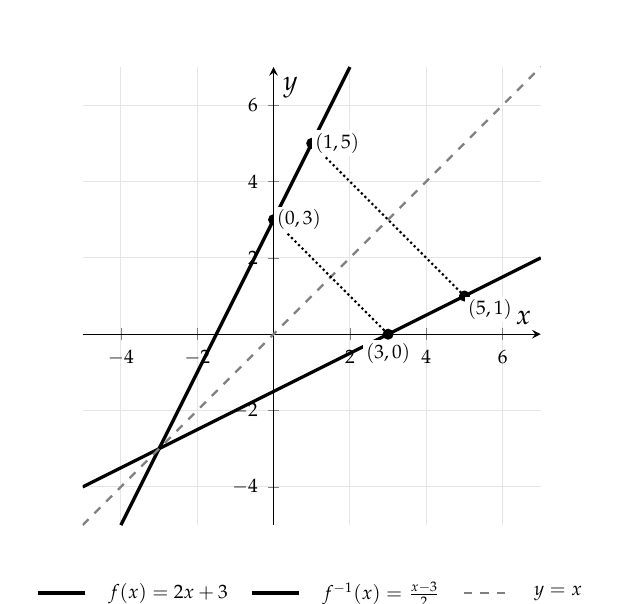
\begin{tikzpicture}
\begin{axis}[width=7.4cm,height=7.4cm,axis lines=middle,xmin=-5,xmax=7,ymin=-5,ymax=7,
  xtick={-4,-2,2,4,6},ytick={-4,-2,2,4,6},grid=major,grid style={gray!20},
  xlabel={$x$},ylabel={$y$},tick label style={font=\scriptsize},
  legend style={at={(0.5,-0.1)},anchor=north,font=\scriptsize,draw=none,legend columns=3,column sep=6pt}]
\addplot[FangBlue,very thick,domain=-4:2]{2*x+3}; \addlegendentry{$f(x)=2x+3$}
\addplot[FangRed,very thick,domain=-5:7]{(x-3)/2}; \addlegendentry{$\finv(x)=\frac{x-3}{2}$}
\addplot[dashed,gray,thick,domain=-5:7]{x}; \addlegendentry{$y=x$}
\draw[densely dotted,thick,FangPurple](axis cs:0,3)--(axis cs:3,0);
\draw[densely dotted,thick,FangPurple](axis cs:1,5)--(axis cs:5,1);
\fill[FangBlue](axis cs:0,3) circle(2pt) node[right,font=\scriptsize,fill=white,inner sep=1pt]{$(0,3)$};
\fill[FangRed](axis cs:3,0) circle(2pt) node[below,font=\scriptsize,fill=white,inner sep=1pt,yshift=-2pt]{$(3,0)$};
\fill[FangBlue](axis cs:1,5) circle(2pt) node[right,font=\scriptsize,fill=white,inner sep=1pt]{$(1,5)$};
\fill[FangRed](axis cs:5,1) circle(2pt) node[below right,font=\scriptsize,fill=white,inner sep=1pt]{$(5,1)$};
\end{axis}
\end{tikzpicture}\\[-2pt]
{\small\textbf{Figure 1.} Each point $(a,b)$ on $f$ has a partner $(b,a)$ on $\finv$.}
\end{minipage}\hfill
\begin{minipage}[t]{0.485\textwidth}\centering
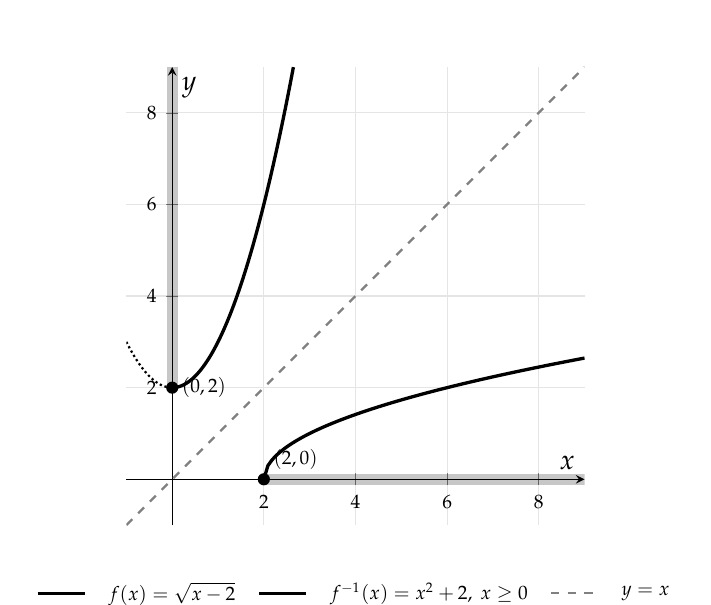
\begin{tikzpicture}
\begin{axis}[width=7.4cm,height=7.4cm,axis lines=middle,xmin=-1,xmax=9,ymin=-1,ymax=9,
  xtick={2,4,6,8},ytick={2,4,6,8},grid=major,grid style={gray!20},
  xlabel={$x$},ylabel={$y$},tick label style={font=\scriptsize},
  legend style={at={(0.5,-0.1)},anchor=north,font=\scriptsize,draw=none,legend columns=3,column sep=6pt}]
\draw[FangBlue,line width=4pt,opacity=0.22](axis cs:2,0)--(axis cs:9,0);
\draw[FangRed,line width=4pt,opacity=0.22](axis cs:0,2)--(axis cs:0,9);
\addplot[FangBlue,very thick,domain=2:9,samples=80]{sqrt(x-2)}; \addlegendentry{$f(x)=\sqrt{x-2}$}
\addplot[FangRed,very thick,domain=0:2.645,samples=60]{x^2+2}; \addlegendentry{$\finv(x)=x^2+2,\ x\ge0$}
\addplot[dashed,gray,thick,domain=-1:9]{x}; \addlegendentry{$y=x$}
\addplot[FangRed,thick,densely dotted,domain=-1:0,samples=30]{x^2+2};
\fill[FangBlue](axis cs:2,0) circle(2.2pt) node[above right,font=\scriptsize]{$(2,0)$};
\fill[FangRed](axis cs:0,2) circle(2.2pt) node[right,font=\scriptsize]{$(0,2)$};
\end{axis}
\end{tikzpicture}\\[-2pt]
{\small\textbf{Figure 2.} Shaded strips: domain of $f$ (blue) and range of $\finv$ (red).}
\end{minipage}
\end{center}

\begin{multicols}{2}
\textbf{Fold the paper along $y=x$:} the graph of $f$ lands exactly on the graph of $\finv$.\par
\textbf{Why?} The points $(a,b)$ and $(b,a)$ are mirror images in $y=x$:
\begin{itemize}[leftmargin=*,itemsep=1pt,topsep=2pt]
\item their midpoint $\left(\frac{a+b}{2},\frac{a+b}{2}\right)$ \textbf{lies on} $y=x$;
\item the segment joining them has slope $\frac{a-b}{b-a}=-1$, so it is \textbf{perpendicular} to $y=x$.
\end{itemize}
Every point of $f$ is reflected, so the whole graph is reflected. \textbf{Slope bonus:} $2$ and $\tfrac12$ are reciprocals — steep becomes flat.
\columnbreak

\textbf{Domain and range trade places, too} (Figure 2). \par
$f(x)=\sqrt{x-2}$: domain $[2,\infty)$, range $[0,\infty)$. \par
$\finv(x)=x^2+2$, $x\ge0$: domain $[0,\infty)$, range $[2,\infty)$. \par
The dotted left half of the parabola is \textbf{not} part of $\finv$ — it is not the mirror image of any point of $f$. That is why we wrote ``$x\ge0$'' in Example~3.
\end{multicols}

% ======================= PART 4 =======================
\sect{4}{Domain and range of the inverse}

\begin{idea}[The rule]
\[ \text{Domain of } \finv = \text{Range of } f \qquad\qquad \text{Range of } \finv = \text{Domain of } f \]
Reason: $\finv$ uses the outputs of $f$ as its inputs, and gives back the inputs of $f$ as its outputs.
\end{idea}

\textbf{How to find them — the safe method}
\begin{enumerate}[leftmargin=*,itemsep=2pt]
\item Find the domain and range of $f$ \textbf{first} (look at the graph, or ask ``which $x$ are allowed?'' and ``which $y$ can come out?'').
\item \textbf{Swap} them: that gives the domain and range of $\finv$.
\item Find the formula for $\finv$, then \textbf{attach the domain from step 2} to it.
\end{enumerate}

\begin{warn}
\textbf{Don't trust the formula alone.} In Example 3 the formula $x^2+2$ works for every real $x$, but the inverse only has domain $[0,\infty)$ — because that is the range of $f(x)=\sqrt{x-2}$. Always get the domain of $\finv$ from the range of $f$.
\end{warn}

\begin{example}[Example 4 \;·\; rational function]
$f(x)=\dfrac{2x+1}{x-3}$: domain $x\neq3$ (can't divide by $0$). Horizontal asymptote $y=\frac{2}{1}=2$, and $f(x)=2$ has no solution, so range $y\neq2$.\par
Therefore $\finv(x)=\dfrac{3x+1}{x-2}$ has \textbf{domain} $x\neq2$ and \textbf{range} $y\neq3$. The formula agrees: it is undefined at $x=2$, and its horizontal asymptote is $y=3$. \checkmark
\end{example}

\begin{example}[Example 5 \;·\; when there is no inverse — restrict the domain]
$f(x)=x^2$ is \textbf{not one-to-one}: $f(2)=f(-2)=4$, so $\finv(4)$ would have to be both $2$ and $-2$. On the graph, the horizontal line $y=4$ hits the parabola twice (\textbf{horizontal line test} fails).\par
Fix: keep only half. With domain $x\ge0$: range $[0,\infty)$, so $\finv(x)=\sqrt{x}$ with domain $[0,\infty)$ and range $[0,\infty)$.\par
With domain $x\le0$ instead: $\finv(x)=-\sqrt{x}$, domain $[0,\infty)$, range $(-\infty,0]$.
\end{example}

\begin{center}
\renewcommand{\arraystretch}{1.25}
\begin{tabular}{@{}lll@{}}
\toprule
\textbf{Question} & \textbf{About $f$} & \textbf{About $\finv$}\\ \midrule
Point & $(a,b)$ & $(b,a)$\\
Domain & $D$ & the range of $f$\\
Range & $R$ & the domain of $f$\\
Graph & — & reflection of $f$ over $y=x$\\
Exists? & only if $f$ is one-to-one & passes the horizontal line test\\
Proof & \multicolumn{2}{l}{$f(\finv(x))=x$ \textbf{and} $\finv(f(x))=x$}\\
\bottomrule
\end{tabular}
\end{center}

% ======================= PRACTICE =======================
\newpage
\sect{5}{Practice}
\ifkey\else\textit{Show your work. When you find an inverse, do a simple-case check: pick an easy $x$, find $f(x)$, and make sure $\finv$ sends it back.}\fi

\medskip
\needspace{6cm}{\large\bfseries\color{FangBlue}A.\ Warm-up} \easy

\begin{enumerate}[leftmargin=*,label=\textbf{\arabic*.},itemsep=6pt]
\np\item If $f(3)=7$, what is $\finv(7)$? \hfill If $\finv(-2)=5$, what is $f(5)$?
\work[1.2cm]{$\finv(7)=3$ (because $f$ sends $3$ to $7$). \quad $f(5)=-2$ (because $\finv$ sends $-2$ to $5$, so $f$ sends $5$ to $-2$).}

\np\item The table shows $f$. Find $\finv(11)$ and $\finv(5)$, and make a table for $\finv$.
\qquad\begin{tabular}{c|cccc}$x$&1&2&3&4\\\hline $f(x)$&5&8&11&14\end{tabular}
\work[1.6cm]{$\finv(11)=3$, \; $\finv(5)=1$. \quad Table of $\finv$: \; $x$: $5,8,11,14$ \;$\to$\; $\finv(x)$: $1,2,3,4$. \\ (Here $f(x)=3x+2$, so $\finv(x)=\frac{x-2}{3}$.)}

\np\item Find $\finv(x)$ for $f(x)=4x-5$.
\work[2.2cm]{$y=4x-5$ \;$\to$\; swap: $x=4y-5$ \;$\to$\; $x+5=4y$ \;$\to$\; $\finv(x)=\dfrac{x+5}{4}$. \; Check: $f(2)=3$, $\finv(3)=2$ \checkmark}

\np\item Find $\finv(x)$ for $f(x)=\dfrac{x+6}{3}$.
\work[2.2cm]{Swap: $x=\dfrac{y+6}{3}$ \;$\to$\; $3x=y+6$ \;$\to$\; $\finv(x)=3x-6$. \; Check: $f(0)=2$, $\finv(2)=0$ \checkmark}
\end{enumerate}

\needspace{6cm}{\large\bfseries\color{FangBlue}B.\ Prove it (check both orders)} \medium

\begin{enumerate}[resume,leftmargin=*,label=\textbf{\arabic*.},itemsep=6pt]
\np\item Prove that $f(x)=3x-7$ and $g(x)=\dfrac{x+7}{3}$ are inverses.
\work[2.6cm]{$f(g(x))=3\cdot\dfrac{x+7}{3}-7=x+7-7=x$. \quad $g(f(x))=\dfrac{(3x-7)+7}{3}=\dfrac{3x}{3}=x$. \\ Both are $x$ for all real $x$, so they are inverses. $\blacksquare$}

\np\item Are $f(x)=x^3+1$ and $g(x)=\sqrt[3]{x-1}$ inverses? Prove your answer.
\work[2.6cm]{$f(g(x))=\big(\sqrt[3]{x-1}\big)^3+1=(x-1)+1=x$. \quad $g(f(x))=\sqrt[3]{(x^3+1)-1}=\sqrt[3]{x^3}=x$. \\ Yes — both orders give $x$ for every real $x$ (cube roots work for negatives too). $\blacksquare$}

\np\item Are $f(x)=2x+4$ and $g(x)=\dfrac{x}{2}-4$ inverses? Prove your answer.
\work[2.4cm]{$f(g(x))=2\left(\dfrac{x}{2}-4\right)+4=x-8+4=x-4\neq x$. \; \textbf{Not} inverses (one failed composition is enough). \\ Simple case: $f(0)=4$ but $g(4)=-2\neq0$. The real inverse is $\finv(x)=\dfrac{x-4}{2}=\dfrac{x}{2}-2$.}
\end{enumerate}

\needspace{6cm}{\large\bfseries\color{FangBlue}C.\ Domain and range of $f$ and $\finv$} \medium\ \hard

\needspace{6cm}\textit{For each function: (a) domain and range of $f$, (b) the formula for $\finv$, (c) domain and range of $\finv$.}

\begin{enumerate}[resume,leftmargin=*,label=\textbf{\arabic*.},itemsep=6pt]
\np\item \medium\ $f(x)=\sqrt{x+3}$
\work[3.2cm]{(a) Domain $[-3,\infty)$ (need $x+3\ge0$); range $[0,\infty)$. \\
(b) Swap: $x=\sqrt{y+3}$ \;$\to$\; $x^2=y+3$ \;$\to$\; $\finv(x)=x^2-3$, \; $x\ge0$. \\
(c) Domain of $\finv$ $=[0,\infty)$ (the range of $f$); range of $\finv$ $=[-3,\infty)$ (the domain of $f$). \\
Check: $f(1)=2$, \; $\finv(2)=4-3=1$ \checkmark}

\np\item \medium\ $f(x)=(x-2)^2+1$, \; $x\ge2$
\work[3.2cm]{(a) Domain $[2,\infty)$ (given); the vertex is $(2,1)$ and the graph goes up, so range $[1,\infty)$. \\
(b) Swap: $x=(y-2)^2+1$ \;$\to$\; $(y-2)^2=x-1$ \;$\to$\; $y-2=\sqrt{x-1}$ (take $+$, because $y\ge2$) \;$\to$\; $\finv(x)=2+\sqrt{x-1}$. \\
(c) Domain of $\finv$ $=[1,\infty)$; range $=[2,\infty)$. \quad Check: $f(4)=5$, \; $\finv(5)=2+2=4$ \checkmark}

\np\item \medium\ $f(x)=\dfrac{x+1}{x-4}$
\work[3.4cm]{(a) Domain $x\neq4$. Horizontal asymptote $y=1$ and $f(x)=1$ has no solution, so range $y\neq1$. \\
(b) Swap: $x=\dfrac{y+1}{y-4}$ \;$\to$\; $xy-4x=y+1$ \;$\to$\; $xy-y=4x+1$ \;$\to$\; $y(x-1)=4x+1$ \;$\to$\; $\finv(x)=\dfrac{4x+1}{x-1}$. \\
(c) Domain of $\finv$: $x\neq1$; range: $y\neq4$ — exactly the range and domain of $f$ swapped. \quad Check: $f(5)=6$, $\finv(6)=\frac{25}{5}=5$ \checkmark}

\np\item \hard\ $f(x)=-\sqrt{4-x}$
\work[3.4cm]{(a) Need $4-x\ge0$: domain $(-\infty,4]$. A square root is $\ge0$, so with the minus sign: range $(-\infty,0]$. \\
(b) Swap: $x=-\sqrt{4-y}$ \;$\to$\; square: $x^2=4-y$ \;$\to$\; $\finv(x)=4-x^2$, \; $x\le0$. \\
(c) Domain of $\finv$ $=(-\infty,0]$; range $=(-\infty,4]$. \quad Check: $f(0)=-2$, \; $\finv(-2)=4-4=0$ \checkmark \\
(Without ``$x\le0$'' the formula would be a whole parabola — wrong.)}

\np\item \hard\ $f(x)=x^2-6x$ is not one-to-one. Restrict its domain to the largest interval that contains $x=5$ on which $f$ \emph{is} one-to-one. Then find $\finv$ with its domain and range.
\work[3.8cm]{Complete the square: $f(x)=(x-3)^2-9$, vertex $(3,-9)$. Each side of $x=3$ is one-to-one; the side containing $5$ is $x\ge3$. \\
$f$: domain $[3,\infty)$, range $[-9,\infty)$. \\
Swap: $x=(y-3)^2-9$ \;$\to$\; $(y-3)^2=x+9$ \;$\to$\; $y=3+\sqrt{x+9}$ (take $+$ because $y\ge3$). \\
$\finv(x)=3+\sqrt{x+9}$: domain $[-9,\infty)$, range $[3,\infty)$. \quad Check: $f(5)=-5$, \; $\finv(-5)=3+2=5$ \checkmark}
\end{enumerate}

\needspace{6cm}{\large\bfseries\color{FangBlue}D.\ Graphs} \medium

\begin{enumerate}[resume,leftmargin=*,label=\textbf{\arabic*.},itemsep=6pt]
\np\item The graph of $f$ is shown (blue, through $(-4,-3)$, $(-2,-2)$, $(0,0)$, $(2,4)$). Draw $y=x$, then sketch $\finv$ by swapping the coordinates of each marked point. State the domain and range of $f$ and of $\finv$.

\begin{center}
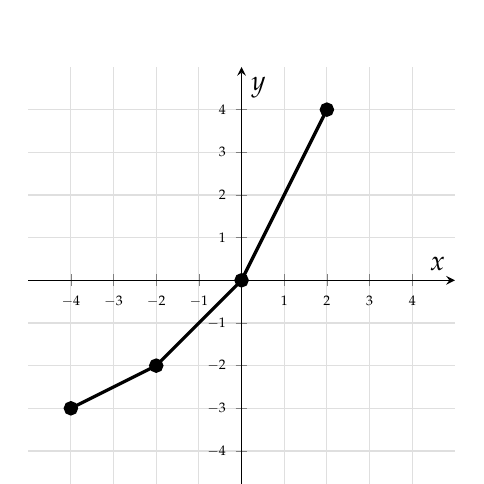
\begin{tikzpicture}
\begin{axis}[width=7cm,height=7cm,axis lines=middle,xmin=-5,xmax=5,ymin=-5,ymax=5,
  xtick={-4,...,4},ytick={-4,...,4},grid=both,grid style={gray!25},xlabel={$x$},ylabel={$y$},tick label style={font=\tiny}]
\addplot[FangBlue,very thick,mark=*,mark options={fill=FangBlue}] coordinates {(-4,-3)(-2,-2)(0,0)(2,4)};
\ifkey
\addplot[dashed,gray,thick,domain=-5:5]{x};
\addplot[FangRed,very thick,mark=*,mark options={fill=FangRed}] coordinates {(-3,-4)(-2,-2)(0,0)(4,2)};
\fi
\end{axis}
\end{tikzpicture}
\end{center}
\work[1.2cm]{$\finv$ (red) goes through $(-3,-4)$, $(-2,-2)$, $(0,0)$, $(4,2)$. Points on $y=x$, like $(-2,-2)$ and $(0,0)$, stay put. \\
$f$: domain $[-4,2]$, range $[-3,4]$. \quad $\finv$: domain $[-3,4]$, range $[-4,2]$.}

\np\item (a) The point $(-4,\,1)$ is on the graph of $f$. Which point must be on the graph of $\finv$? \\
(b) For $f(x)=2x-3$, find the point where the graphs of $f$ and $\finv$ cross.
\work[2.4cm]{(a) $(1,\,-4)$ — swap the coordinates. \\
(b) $\finv(x)=\dfrac{x+3}{2}$. The graphs are mirror images in $y=x$, so (for an increasing line) they meet on $y=x$: solve $2x-3=x$, so $x=3$. The point is $(3,3)$. Check: $f(3)=3$ and $\finv(3)=3$ \checkmark}
\end{enumerate}

\needspace{6cm}{\large\bfseries\color{FangBlue}E.\ Challenge} \hard

\begin{enumerate}[resume,leftmargin=*,label=\textbf{\arabic*.},itemsep=6pt]
\np\item Show that $f(x)=\dfrac{3x+2}{x-3}$ is its own inverse. What does that tell you about its graph?
\work[3.4cm]{$f(f(x))=\dfrac{3\cdot\frac{3x+2}{x-3}+2}{\frac{3x+2}{x-3}-3}=\dfrac{\frac{9x+6+2x-6}{x-3}}{\frac{3x+2-3x+9}{x-3}}=\dfrac{11x}{11}=x$ \; for $x\neq3$. \\
So $\finv=f$. Its graph is symmetric about the line $y=x$ (reflecting it changes nothing). Also: domain $x\neq3$ and range $y\neq3$ are the same set, as they must be.}

\np\item Explain why $f(x)=x^2$ has no inverse on all real numbers, but $g(x)=x^2$, $x\ge0$, does. Give the domain and range of $g^{-1}$.
\work[2.6cm]{$f(-2)=f(2)=4$: two inputs give the same output, so ``undo'' would have to send $4$ to two places — not a function (horizontal line test fails). Restricting to $x\ge0$ keeps each output only once. \\
$g^{-1}(x)=\sqrt{x}$: domain $[0,\infty)$ (range of $g$), range $[0,\infty)$ (domain of $g$).}
\end{enumerate}

\ifkey\else
\vfill
\begin{simple}
\textbf{Before you hand it in:} for every inverse you found, did you (1) check one easy number both ways, and (2) write the domain of $\finv$ as the \textbf{range of} $f$?
\end{simple}
\fi

\end{document}
"
% =====================================================================
\documentclass[11pt,letterpaper]{article}
\usepackage[margin=0.8in,top=0.85in,bottom=0.8in]{geometry}
\usepackage{mathpazo}
\usepackage[T1]{fontenc}
\usepackage{amsmath,amssymb}
\usepackage{xcolor}
\usepackage{enumitem}
\usepackage{multicol}
\usepackage{booktabs}
\usepackage{needspace}
\usepackage{fancyhdr}
\usepackage[most]{tcolorbox}
\usepackage{pgfplots}
\pgfplotsset{compat=1.17}
\usetikzlibrary{arrows.meta}

\definecolor{FangBlue}{HTML}{1F4E79}
\definecolor{FangTeal}{HTML}{0F7C7C}
\definecolor{FangGold}{HTML}{C9962B}
\definecolor{FangRed}{HTML}{B3261E}
\definecolor{FangGreen}{HTML}{2E8B57}
\definecolor{FangPurple}{HTML}{6A4BD8}
\definecolor{Soft}{HTML}{F4F7FB}
% black-and-white version: pdflatex with \def\isbw{1} before \input
\ifdefined\isbw
\definecolor{FangBlue}{HTML}{000000}\definecolor{FangTeal}{HTML}{000000}\definecolor{FangGold}{HTML}{555555}
\definecolor{FangRed}{HTML}{000000}\definecolor{FangGreen}{HTML}{000000}\definecolor{FangPurple}{HTML}{000000}\definecolor{Soft}{HTML}{FFFFFF}
\fi

\newif\ifkey
\ifdefined\iskey \keytrue \else \keyfalse \fi

\pagestyle{fancy}\fancyhf{}
\renewcommand{\headrulewidth}{0.4pt}
\fancyhead[L]{\small\color{FangBlue}\textbf{Prof. Fang Math} \,|\, Algebra 2 \,·\, 6-7 Inverse Relations \& Functions}
\fancyhead[R]{\small\ifkey\textcolor{FangRed}{\textbf{ANSWER KEY}}\else Name: \underline{\hspace{4.2cm}}\fi}
\fancyfoot[C]{\small\thepage}
\fancyfoot[R]{\scriptsize\color{gray}fangmath.com}
\setlength{\headheight}{14pt}
\setlength{\parindent}{0pt}
\setlength{\parskip}{4pt}

% ---------- boxes ----------
\newtcolorbox{idea}[1][]{colback=Soft,colframe=FangBlue,boxrule=0.8pt,arc=3pt,left=8pt,right=8pt,top=6pt,bottom=6pt,
  fonttitle=\bfseries,coltitle=white,colbacktitle=FangBlue,title={#1}}
\newtcolorbox{example}[1][]{colback=white,colframe=FangTeal,boxrule=0.6pt,arc=3pt,left=8pt,right=8pt,top=5pt,bottom=5pt,
  fonttitle=\bfseries,coltitle=FangTeal,colbacktitle=white,title={#1},attach boxed title to top left={xshift=8pt,yshift=-7pt},boxed title style={boxrule=0pt,colframe=white}, enhanced}
\newtcolorbox{warn}{colback=FangRed!5,colframe=FangRed,boxrule=0.6pt,arc=3pt,left=8pt,right=8pt,top=4pt,bottom=4pt,leftrule=3pt}
\newtcolorbox{simple}{colback=FangGold!10,colframe=FangGold,boxrule=0.6pt,arc=3pt,left=8pt,right=8pt,top=4pt,bottom=4pt,leftrule=3pt}
\newtcolorbox{sol}{colback=FangGreen!6,colframe=FangGreen,boxrule=0.5pt,arc=2pt,left=6pt,right=6pt,top=3pt,bottom=3pt,breakable}

\newcommand{\badge}[2]{\tcbox[on line,colback=#1,colframe=#1,coltext=white,boxrule=0pt,arc=6pt,left=4pt,right=4pt,top=1pt,bottom=1pt,fontupper=\scriptsize\bfseries]{#2}}
\newcommand{\easy}{\badge{FangGreen}{EASY}}
\newcommand{\medium}{\badge{FangTeal}{MEDIUM}}
\newcommand{\hard}{\badge{FangRed}{HARD}}
\newcommand{\finv}{f^{-1}}
\newcommand{\work}[2][]{\ifkey\begin{sol}#2\end{sol}\else\vspace*{#1}\fi}
\newcommand{\np}[1][6cm]{\needspace{#1}}
\newcommand{\sect}[2]{\par\needspace{7cm}\medskip{\Large\bfseries\color{FangBlue}\tcbox[on line,colback=FangBlue,colframe=FangBlue,coltext=white,arc=2pt,boxrule=0pt,left=5pt,right=5pt,top=1pt,bottom=1pt]{#1}\ #2}\par\smallskip}

\begin{document}

% ======================= TITLE =======================
\begin{center}
{\color{FangBlue}\Huge\bfseries Inverse Functions}\\[2pt]
{\large Undo the function — find it, prove it, graph it, and get its domain \& range}
\ifkey\\[3pt]{\color{FangRed}\large\bfseries Answer Key with complete solutions}\fi
\end{center}
\vspace{-4pt}

\begin{idea}[The big idea]
A function $f$ takes an input $x$ to an output $y$. Its \textbf{inverse} $\finv$ goes back: it takes $y$ to $x$.
\[ x \xrightarrow{\;\;f\;\;} y \qquad\qquad y \xrightarrow{\;\;\finv\;\;} x \qquad\qquad\text{so}\qquad f(a)=b \iff \finv(b)=a. \]
Every point $(a,b)$ on $f$ becomes the point $(b,a)$ on $\finv$: \textbf{inputs and outputs trade places.}
\end{idea}

\begin{simple}
\textbf{Simple case first.} ``Add $3$'' is undone by ``subtract $3$'': if $f(x)=x+3$ then $\finv(x)=x-3$. Check: $f(4)=7$ and $\finv(7)=4$.\par
``Double, then add $3$'' is undone by doing the opposite steps in the \textbf{opposite order}: subtract $3$, then halve. Like putting on socks then shoes — you take off the shoes first.
\end{simple}

\begin{center}
\begin{tabular}{c|cccc}
\toprule
$x$ & $0$ & $1$ & $2$ & $3$\\ \midrule
$f(x)=2x+3$ & $3$ & $5$ & $7$ & $9$\\
\bottomrule
\end{tabular}
\qquad$\Longrightarrow$\qquad
\begin{tabular}{c|cccc}
\toprule
$x$ & $3$ & $5$ & $7$ & $9$\\ \midrule
$\finv(x)$ & $0$ & $1$ & $2$ & $3$\\
\bottomrule
\end{tabular}
\end{center}

\begin{warn}
\textbf{Watch out:} $\finv(x)$ means the \emph{inverse function}. It is \textbf{not} $\dfrac{1}{f(x)}$. The $-1$ is not an exponent here.
\end{warn}

% ======================= PART 1 =======================
\sect{1}{How to find the inverse — four steps}

\begin{multicols}{2}
\begin{enumerate}[leftmargin=*,itemsep=2pt]
\item Replace $f(x)$ with $y$.
\item \textbf{Swap} $x$ and $y$.
\item \textbf{Solve} for $y$.
\item Replace $y$ with $\finv(x)$ and \textbf{state its domain}.
\end{enumerate}
\columnbreak
Step 2 is the whole idea: swapping $x$ and $y$ is exactly ``inputs and outputs trade places.'' Steps 3 and 4 just tidy up the answer.
\end{multicols}

\begin{example}[Example 1 \;·\; a line]
Find the inverse of $f(x)=2x+3$.\par
\begin{tabular}{@{}ll@{}}
$y = 2x+3$ & Step 1\\
$x = 2y+3$ & Step 2: swap\\
$x-3 = 2y \;\Rightarrow\; y=\dfrac{x-3}{2}$ & Step 3: solve\\[6pt]
$\finv(x)=\dfrac{x-3}{2}$, \; domain: all real numbers & Step 4
\end{tabular}\par
\textbf{Simple case check:} $f(1)=5$, and $\finv(5)=\frac{5-3}{2}=1$. \checkmark
\end{example}

\begin{example}[Example 2 \;·\; a rational function]
Find the inverse of $f(x)=\dfrac{2x+1}{x-3}$.\par
Swap: $x=\dfrac{2y+1}{y-3}$. \; Multiply by $(y-3)$: $xy-3x=2y+1$. \; Collect the $y$ terms on one side: $xy-2y=3x+1$.\par
Factor out $y$: $y(x-2)=3x+1$, so
\[\finv(x)=\frac{3x+1}{x-2},\qquad x\neq 2.\]
\textbf{Simple case check:} $f(4)=\frac{9}{1}=9$, and $\finv(9)=\frac{28}{7}=4$. \checkmark
\end{example}

\begin{example}[Example 3 \;·\; a square root — the domain matters]
Find the inverse of $f(x)=\sqrt{x-2}$.\par
Swap: $x=\sqrt{y-2}$. Square both sides: $x^2=y-2$, so $y=x^2+2$.\par
\textbf{But} $x$ here was a square-root output, and square roots are never negative, so $x\ge 0$:
\[\finv(x)=x^2+2,\qquad x\ge 0.\]
Without ``$x\ge0$'' you would get a whole parabola, which is \emph{not} the inverse (see the graph in Part~3).
\end{example}

% ======================= PART 2 =======================
\sect{2}{How to prove two functions are inverses}

\begin{idea}[The test — you must check BOTH orders]
$f$ and $g$ are inverse functions exactly when
\[ f\big(g(x)\big)=x \ \text{ for every } x \text{ in the domain of } g \qquad\text{and}\qquad g\big(f(x)\big)=x \ \text{ for every } x \text{ in the domain of } f. \]
In words: doing one and then the other \textbf{always brings you back to where you started}.
\end{idea}

\textbf{Why this is the right test.} Suppose $f(a)=b$. If $g$ undoes $f$, then $g(b)=a$, i.e.\ $g(f(a))=a$. The same thinking with the roles switched gives $f(g(b))=b$. So ``undoing'' means exactly the two equations above.

\begin{example}[Proof 1 \;·\; $f(x)=2x+3$ and $g(x)=\dfrac{x-3}{2}$]
\[ f\big(g(x)\big)=2\cdot\frac{x-3}{2}+3=(x-3)+3=x. \qquad
   g\big(f(x)\big)=\frac{(2x+3)-3}{2}=\frac{2x}{2}=x. \]
Both compositions equal $x$ for all real $x$, so $g=\finv$. \qquad $\blacksquare$
\end{example}

\begin{example}[Proof 2 \;·\; $f(x)=\dfrac{2x+1}{x-3}$ and $g(x)=\dfrac{3x+1}{x-2}$]
\[ f\big(g(x)\big)=\frac{2\cdot\frac{3x+1}{x-2}+1}{\frac{3x+1}{x-2}-3}
 =\frac{\frac{2(3x+1)+(x-2)}{x-2}}{\frac{(3x+1)-3(x-2)}{x-2}}
 =\frac{6x+2+x-2}{3x+1-3x+6}=\frac{7x}{7}=x \quad (x\neq2). \]
\[ g\big(f(x)\big)=\frac{3\cdot\frac{2x+1}{x-3}+1}{\frac{2x+1}{x-3}-2}
 =\frac{\frac{3(2x+1)+(x-3)}{x-3}}{\frac{(2x+1)-2(x-3)}{x-3}}
 =\frac{6x+3+x-3}{2x+1-2x+6}=\frac{7x}{7}=x \quad (x\neq3). \]
Both orders give $x$, so they are inverses. \qquad $\blacksquare$
\end{example}

\begin{warn}
\textbf{Why one order is not enough.} Take $f(x)=x^2$ and $g(x)=\sqrt{x}$. Then $f(g(x))=(\sqrt x)^2=x$ for $x\ge0$ — looks fine. But $g(f(x))=\sqrt{x^2}=|x|$, and $g(f(-3))=3\neq-3$. So they are \textbf{not} inverses — unless we restrict $f$ to $x\ge0$ (Part 4).
\end{warn}

% ======================= PART 3 =======================
\sect{3}{The graph: a mirror image over the line $y=x$}

\begin{center}
\begin{minipage}[t]{0.485\textwidth}\centering
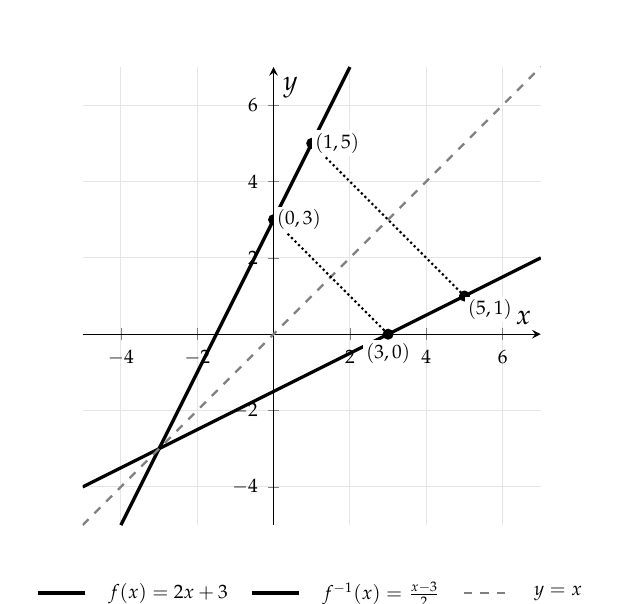
\begin{tikzpicture}
\begin{axis}[width=7.4cm,height=7.4cm,axis lines=middle,xmin=-5,xmax=7,ymin=-5,ymax=7,
  xtick={-4,-2,2,4,6},ytick={-4,-2,2,4,6},grid=major,grid style={gray!20},
  xlabel={$x$},ylabel={$y$},tick label style={font=\scriptsize},
  legend style={at={(0.5,-0.1)},anchor=north,font=\scriptsize,draw=none,legend columns=3,column sep=6pt}]
\addplot[FangBlue,very thick,domain=-4:2]{2*x+3}; \addlegendentry{$f(x)=2x+3$}
\addplot[FangRed,very thick,domain=-5:7]{(x-3)/2}; \addlegendentry{$\finv(x)=\frac{x-3}{2}$}
\addplot[dashed,gray,thick,domain=-5:7]{x}; \addlegendentry{$y=x$}
\draw[densely dotted,thick,FangPurple](axis cs:0,3)--(axis cs:3,0);
\draw[densely dotted,thick,FangPurple](axis cs:1,5)--(axis cs:5,1);
\fill[FangBlue](axis cs:0,3) circle(2pt) node[right,font=\scriptsize,fill=white,inner sep=1pt]{$(0,3)$};
\fill[FangRed](axis cs:3,0) circle(2pt) node[below,font=\scriptsize,fill=white,inner sep=1pt,yshift=-2pt]{$(3,0)$};
\fill[FangBlue](axis cs:1,5) circle(2pt) node[right,font=\scriptsize,fill=white,inner sep=1pt]{$(1,5)$};
\fill[FangRed](axis cs:5,1) circle(2pt) node[below right,font=\scriptsize,fill=white,inner sep=1pt]{$(5,1)$};
\end{axis}
\end{tikzpicture}\\[-2pt]
{\small\textbf{Figure 1.} Each point $(a,b)$ on $f$ has a partner $(b,a)$ on $\finv$.}
\end{minipage}\hfill
\begin{minipage}[t]{0.485\textwidth}\centering
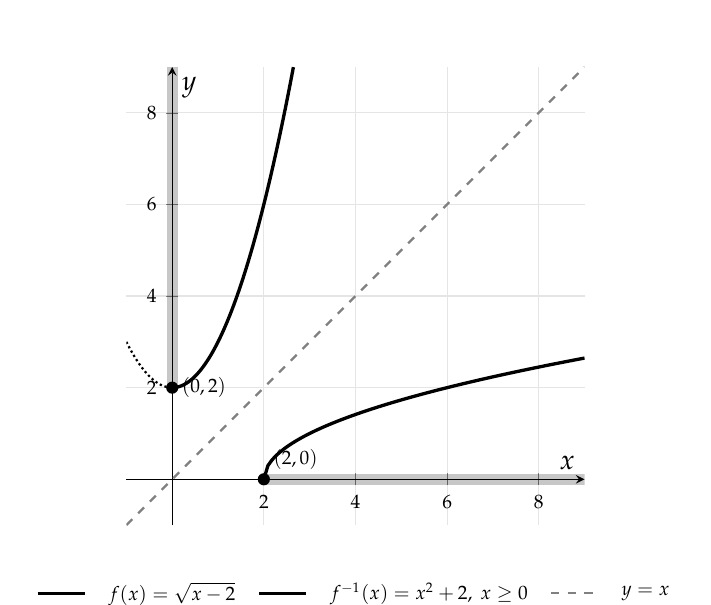
\begin{tikzpicture}
\begin{axis}[width=7.4cm,height=7.4cm,axis lines=middle,xmin=-1,xmax=9,ymin=-1,ymax=9,
  xtick={2,4,6,8},ytick={2,4,6,8},grid=major,grid style={gray!20},
  xlabel={$x$},ylabel={$y$},tick label style={font=\scriptsize},
  legend style={at={(0.5,-0.1)},anchor=north,font=\scriptsize,draw=none,legend columns=3,column sep=6pt}]
\draw[FangBlue,line width=4pt,opacity=0.22](axis cs:2,0)--(axis cs:9,0);
\draw[FangRed,line width=4pt,opacity=0.22](axis cs:0,2)--(axis cs:0,9);
\addplot[FangBlue,very thick,domain=2:9,samples=80]{sqrt(x-2)}; \addlegendentry{$f(x)=\sqrt{x-2}$}
\addplot[FangRed,very thick,domain=0:2.645,samples=60]{x^2+2}; \addlegendentry{$\finv(x)=x^2+2,\ x\ge0$}
\addplot[dashed,gray,thick,domain=-1:9]{x}; \addlegendentry{$y=x$}
\addplot[FangRed,thick,densely dotted,domain=-1:0,samples=30]{x^2+2};
\fill[FangBlue](axis cs:2,0) circle(2.2pt) node[above right,font=\scriptsize]{$(2,0)$};
\fill[FangRed](axis cs:0,2) circle(2.2pt) node[right,font=\scriptsize]{$(0,2)$};
\end{axis}
\end{tikzpicture}\\[-2pt]
{\small\textbf{Figure 2.} Shaded strips: domain of $f$ (blue) and range of $\finv$ (red).}
\end{minipage}
\end{center}

\begin{multicols}{2}
\textbf{Fold the paper along $y=x$:} the graph of $f$ lands exactly on the graph of $\finv$.\par
\textbf{Why?} The points $(a,b)$ and $(b,a)$ are mirror images in $y=x$:
\begin{itemize}[leftmargin=*,itemsep=1pt,topsep=2pt]
\item their midpoint $\left(\frac{a+b}{2},\frac{a+b}{2}\right)$ \textbf{lies on} $y=x$;
\item the segment joining them has slope $\frac{a-b}{b-a}=-1$, so it is \textbf{perpendicular} to $y=x$.
\end{itemize}
Every point of $f$ is reflected, so the whole graph is reflected. \textbf{Slope bonus:} $2$ and $\tfrac12$ are reciprocals — steep becomes flat.
\columnbreak

\textbf{Domain and range trade places, too} (Figure 2). \par
$f(x)=\sqrt{x-2}$: domain $[2,\infty)$, range $[0,\infty)$. \par
$\finv(x)=x^2+2$, $x\ge0$: domain $[0,\infty)$, range $[2,\infty)$. \par
The dotted left half of the parabola is \textbf{not} part of $\finv$ — it is not the mirror image of any point of $f$. That is why we wrote ``$x\ge0$'' in Example~3.
\end{multicols}

% ======================= PART 4 =======================
\sect{4}{Domain and range of the inverse}

\begin{idea}[The rule]
\[ \text{Domain of } \finv = \text{Range of } f \qquad\qquad \text{Range of } \finv = \text{Domain of } f \]
Reason: $\finv$ uses the outputs of $f$ as its inputs, and gives back the inputs of $f$ as its outputs.
\end{idea}

\textbf{How to find them — the safe method}
\begin{enumerate}[leftmargin=*,itemsep=2pt]
\item Find the domain and range of $f$ \textbf{first} (look at the graph, or ask ``which $x$ are allowed?'' and ``which $y$ can come out?'').
\item \textbf{Swap} them: that gives the domain and range of $\finv$.
\item Find the formula for $\finv$, then \textbf{attach the domain from step 2} to it.
\end{enumerate}

\begin{warn}
\textbf{Don't trust the formula alone.} In Example 3 the formula $x^2+2$ works for every real $x$, but the inverse only has domain $[0,\infty)$ — because that is the range of $f(x)=\sqrt{x-2}$. Always get the domain of $\finv$ from the range of $f$.
\end{warn}

\begin{example}[Example 4 \;·\; rational function]
$f(x)=\dfrac{2x+1}{x-3}$: domain $x\neq3$ (can't divide by $0$). Horizontal asymptote $y=\frac{2}{1}=2$, and $f(x)=2$ has no solution, so range $y\neq2$.\par
Therefore $\finv(x)=\dfrac{3x+1}{x-2}$ has \textbf{domain} $x\neq2$ and \textbf{range} $y\neq3$. The formula agrees: it is undefined at $x=2$, and its horizontal asymptote is $y=3$. \checkmark
\end{example}

\begin{example}[Example 5 \;·\; when there is no inverse — restrict the domain]
$f(x)=x^2$ is \textbf{not one-to-one}: $f(2)=f(-2)=4$, so $\finv(4)$ would have to be both $2$ and $-2$. On the graph, the horizontal line $y=4$ hits the parabola twice (\textbf{horizontal line test} fails).\par
Fix: keep only half. With domain $x\ge0$: range $[0,\infty)$, so $\finv(x)=\sqrt{x}$ with domain $[0,\infty)$ and range $[0,\infty)$.\par
With domain $x\le0$ instead: $\finv(x)=-\sqrt{x}$, domain $[0,\infty)$, range $(-\infty,0]$.
\end{example}

\begin{center}
\renewcommand{\arraystretch}{1.25}
\begin{tabular}{@{}lll@{}}
\toprule
\textbf{Question} & \textbf{About $f$} & \textbf{About $\finv$}\\ \midrule
Point & $(a,b)$ & $(b,a)$\\
Domain & $D$ & the range of $f$\\
Range & $R$ & the domain of $f$\\
Graph & — & reflection of $f$ over $y=x$\\
Exists? & only if $f$ is one-to-one & passes the horizontal line test\\
Proof & \multicolumn{2}{l}{$f(\finv(x))=x$ \textbf{and} $\finv(f(x))=x$}\\
\bottomrule
\end{tabular}
\end{center}

% ======================= PRACTICE =======================
\newpage
\sect{5}{Practice}
\ifkey\else\textit{Show your work. When you find an inverse, do a simple-case check: pick an easy $x$, find $f(x)$, and make sure $\finv$ sends it back.}\fi

\medskip
\needspace{6cm}{\large\bfseries\color{FangBlue}A.\ Warm-up} \easy

\begin{enumerate}[leftmargin=*,label=\textbf{\arabic*.},itemsep=6pt]
\np\item If $f(3)=7$, what is $\finv(7)$? \hfill If $\finv(-2)=5$, what is $f(5)$?
\work[1.2cm]{$\finv(7)=3$ (because $f$ sends $3$ to $7$). \quad $f(5)=-2$ (because $\finv$ sends $-2$ to $5$, so $f$ sends $5$ to $-2$).}

\np\item The table shows $f$. Find $\finv(11)$ and $\finv(5)$, and make a table for $\finv$.
\qquad\begin{tabular}{c|cccc}$x$&1&2&3&4\\\hline $f(x)$&5&8&11&14\end{tabular}
\work[1.6cm]{$\finv(11)=3$, \; $\finv(5)=1$. \quad Table of $\finv$: \; $x$: $5,8,11,14$ \;$\to$\; $\finv(x)$: $1,2,3,4$. \\ (Here $f(x)=3x+2$, so $\finv(x)=\frac{x-2}{3}$.)}

\np\item Find $\finv(x)$ for $f(x)=4x-5$.
\work[2.2cm]{$y=4x-5$ \;$\to$\; swap: $x=4y-5$ \;$\to$\; $x+5=4y$ \;$\to$\; $\finv(x)=\dfrac{x+5}{4}$. \; Check: $f(2)=3$, $\finv(3)=2$ \checkmark}

\np\item Find $\finv(x)$ for $f(x)=\dfrac{x+6}{3}$.
\work[2.2cm]{Swap: $x=\dfrac{y+6}{3}$ \;$\to$\; $3x=y+6$ \;$\to$\; $\finv(x)=3x-6$. \; Check: $f(0)=2$, $\finv(2)=0$ \checkmark}
\end{enumerate}

\needspace{6cm}{\large\bfseries\color{FangBlue}B.\ Prove it (check both orders)} \medium

\begin{enumerate}[resume,leftmargin=*,label=\textbf{\arabic*.},itemsep=6pt]
\np\item Prove that $f(x)=3x-7$ and $g(x)=\dfrac{x+7}{3}$ are inverses.
\work[2.6cm]{$f(g(x))=3\cdot\dfrac{x+7}{3}-7=x+7-7=x$. \quad $g(f(x))=\dfrac{(3x-7)+7}{3}=\dfrac{3x}{3}=x$. \\ Both are $x$ for all real $x$, so they are inverses. $\blacksquare$}

\np\item Are $f(x)=x^3+1$ and $g(x)=\sqrt[3]{x-1}$ inverses? Prove your answer.
\work[2.6cm]{$f(g(x))=\big(\sqrt[3]{x-1}\big)^3+1=(x-1)+1=x$. \quad $g(f(x))=\sqrt[3]{(x^3+1)-1}=\sqrt[3]{x^3}=x$. \\ Yes — both orders give $x$ for every real $x$ (cube roots work for negatives too). $\blacksquare$}

\np\item Are $f(x)=2x+4$ and $g(x)=\dfrac{x}{2}-4$ inverses? Prove your answer.
\work[2.4cm]{$f(g(x))=2\left(\dfrac{x}{2}-4\right)+4=x-8+4=x-4\neq x$. \; \textbf{Not} inverses (one failed composition is enough). \\ Simple case: $f(0)=4$ but $g(4)=-2\neq0$. The real inverse is $\finv(x)=\dfrac{x-4}{2}=\dfrac{x}{2}-2$.}
\end{enumerate}

\needspace{6cm}{\large\bfseries\color{FangBlue}C.\ Domain and range of $f$ and $\finv$} \medium\ \hard

\needspace{6cm}\textit{For each function: (a) domain and range of $f$, (b) the formula for $\finv$, (c) domain and range of $\finv$.}

\begin{enumerate}[resume,leftmargin=*,label=\textbf{\arabic*.},itemsep=6pt]
\np\item \medium\ $f(x)=\sqrt{x+3}$
\work[3.2cm]{(a) Domain $[-3,\infty)$ (need $x+3\ge0$); range $[0,\infty)$. \\
(b) Swap: $x=\sqrt{y+3}$ \;$\to$\; $x^2=y+3$ \;$\to$\; $\finv(x)=x^2-3$, \; $x\ge0$. \\
(c) Domain of $\finv$ $=[0,\infty)$ (the range of $f$); range of $\finv$ $=[-3,\infty)$ (the domain of $f$). \\
Check: $f(1)=2$, \; $\finv(2)=4-3=1$ \checkmark}

\np\item \medium\ $f(x)=(x-2)^2+1$, \; $x\ge2$
\work[3.2cm]{(a) Domain $[2,\infty)$ (given); the vertex is $(2,1)$ and the graph goes up, so range $[1,\infty)$. \\
(b) Swap: $x=(y-2)^2+1$ \;$\to$\; $(y-2)^2=x-1$ \;$\to$\; $y-2=\sqrt{x-1}$ (take $+$, because $y\ge2$) \;$\to$\; $\finv(x)=2+\sqrt{x-1}$. \\
(c) Domain of $\finv$ $=[1,\infty)$; range $=[2,\infty)$. \quad Check: $f(4)=5$, \; $\finv(5)=2+2=4$ \checkmark}

\np\item \medium\ $f(x)=\dfrac{x+1}{x-4}$
\work[3.4cm]{(a) Domain $x\neq4$. Horizontal asymptote $y=1$ and $f(x)=1$ has no solution, so range $y\neq1$. \\
(b) Swap: $x=\dfrac{y+1}{y-4}$ \;$\to$\; $xy-4x=y+1$ \;$\to$\; $xy-y=4x+1$ \;$\to$\; $y(x-1)=4x+1$ \;$\to$\; $\finv(x)=\dfrac{4x+1}{x-1}$. \\
(c) Domain of $\finv$: $x\neq1$; range: $y\neq4$ — exactly the range and domain of $f$ swapped. \quad Check: $f(5)=6$, $\finv(6)=\frac{25}{5}=5$ \checkmark}

\np\item \hard\ $f(x)=-\sqrt{4-x}$
\work[3.4cm]{(a) Need $4-x\ge0$: domain $(-\infty,4]$. A square root is $\ge0$, so with the minus sign: range $(-\infty,0]$. \\
(b) Swap: $x=-\sqrt{4-y}$ \;$\to$\; square: $x^2=4-y$ \;$\to$\; $\finv(x)=4-x^2$, \; $x\le0$. \\
(c) Domain of $\finv$ $=(-\infty,0]$; range $=(-\infty,4]$. \quad Check: $f(0)=-2$, \; $\finv(-2)=4-4=0$ \checkmark \\
(Without ``$x\le0$'' the formula would be a whole parabola — wrong.)}

\np\item \hard\ $f(x)=x^2-6x$ is not one-to-one. Restrict its domain to the largest interval that contains $x=5$ on which $f$ \emph{is} one-to-one. Then find $\finv$ with its domain and range.
\work[3.8cm]{Complete the square: $f(x)=(x-3)^2-9$, vertex $(3,-9)$. Each side of $x=3$ is one-to-one; the side containing $5$ is $x\ge3$. \\
$f$: domain $[3,\infty)$, range $[-9,\infty)$. \\
Swap: $x=(y-3)^2-9$ \;$\to$\; $(y-3)^2=x+9$ \;$\to$\; $y=3+\sqrt{x+9}$ (take $+$ because $y\ge3$). \\
$\finv(x)=3+\sqrt{x+9}$: domain $[-9,\infty)$, range $[3,\infty)$. \quad Check: $f(5)=-5$, \; $\finv(-5)=3+2=5$ \checkmark}
\end{enumerate}

\needspace{6cm}{\large\bfseries\color{FangBlue}D.\ Graphs} \medium

\begin{enumerate}[resume,leftmargin=*,label=\textbf{\arabic*.},itemsep=6pt]
\np\item The graph of $f$ is shown (blue, through $(-4,-3)$, $(-2,-2)$, $(0,0)$, $(2,4)$). Draw $y=x$, then sketch $\finv$ by swapping the coordinates of each marked point. State the domain and range of $f$ and of $\finv$.

\begin{center}
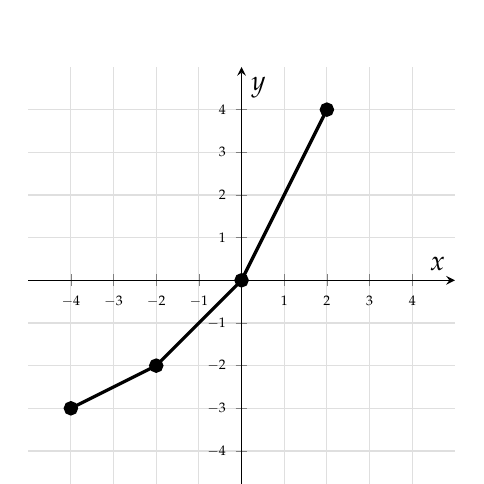
\begin{tikzpicture}
\begin{axis}[width=7cm,height=7cm,axis lines=middle,xmin=-5,xmax=5,ymin=-5,ymax=5,
  xtick={-4,...,4},ytick={-4,...,4},grid=both,grid style={gray!25},xlabel={$x$},ylabel={$y$},tick label style={font=\tiny}]
\addplot[FangBlue,very thick,mark=*,mark options={fill=FangBlue}] coordinates {(-4,-3)(-2,-2)(0,0)(2,4)};
\ifkey
\addplot[dashed,gray,thick,domain=-5:5]{x};
\addplot[FangRed,very thick,mark=*,mark options={fill=FangRed}] coordinates {(-3,-4)(-2,-2)(0,0)(4,2)};
\fi
\end{axis}
\end{tikzpicture}
\end{center}
\work[1.2cm]{$\finv$ (red) goes through $(-3,-4)$, $(-2,-2)$, $(0,0)$, $(4,2)$. Points on $y=x$, like $(-2,-2)$ and $(0,0)$, stay put. \\
$f$: domain $[-4,2]$, range $[-3,4]$. \quad $\finv$: domain $[-3,4]$, range $[-4,2]$.}

\np\item (a) The point $(-4,\,1)$ is on the graph of $f$. Which point must be on the graph of $\finv$? \\
(b) For $f(x)=2x-3$, find the point where the graphs of $f$ and $\finv$ cross.
\work[2.4cm]{(a) $(1,\,-4)$ — swap the coordinates. \\
(b) $\finv(x)=\dfrac{x+3}{2}$. The graphs are mirror images in $y=x$, so (for an increasing line) they meet on $y=x$: solve $2x-3=x$, so $x=3$. The point is $(3,3)$. Check: $f(3)=3$ and $\finv(3)=3$ \checkmark}
\end{enumerate}

\needspace{6cm}{\large\bfseries\color{FangBlue}E.\ Challenge} \hard

\begin{enumerate}[resume,leftmargin=*,label=\textbf{\arabic*.},itemsep=6pt]
\np\item Show that $f(x)=\dfrac{3x+2}{x-3}$ is its own inverse. What does that tell you about its graph?
\work[3.4cm]{$f(f(x))=\dfrac{3\cdot\frac{3x+2}{x-3}+2}{\frac{3x+2}{x-3}-3}=\dfrac{\frac{9x+6+2x-6}{x-3}}{\frac{3x+2-3x+9}{x-3}}=\dfrac{11x}{11}=x$ \; for $x\neq3$. \\
So $\finv=f$. Its graph is symmetric about the line $y=x$ (reflecting it changes nothing). Also: domain $x\neq3$ and range $y\neq3$ are the same set, as they must be.}

\np\item Explain why $f(x)=x^2$ has no inverse on all real numbers, but $g(x)=x^2$, $x\ge0$, does. Give the domain and range of $g^{-1}$.
\work[2.6cm]{$f(-2)=f(2)=4$: two inputs give the same output, so ``undo'' would have to send $4$ to two places — not a function (horizontal line test fails). Restricting to $x\ge0$ keeps each output only once. \\
$g^{-1}(x)=\sqrt{x}$: domain $[0,\infty)$ (range of $g$), range $[0,\infty)$ (domain of $g$).}
\end{enumerate}

\ifkey\else
\vfill
\begin{simple}
\textbf{Before you hand it in:} for every inverse you found, did you (1) check one easy number both ways, and (2) write the domain of $\finv$ as the \textbf{range of} $f$?
\end{simple}
\fi

\end{document}
